% Related publications:
%
% Takasuka et al. (2024), A protocol and analysis of year-long simulations of global storm-resolving models and beyond
% Knight et al. (2024), Cloud properties and boundary layer stability above Southern Ocean sea ice and coastal Antarctica
% Zheng et al. (2024), Using Satellite and ARM Observations to Evaluate Cold Air Outbreak Cloud Transitions in E3SM Global Storm-Resolving Simulations
% Schmidt et al. (2024), Effects of vertical grid spacing on the climate simulated in the ICON-Sapphire global storm-resolving model
% Fons et al. (2024), Investigating the sign of stratocumulus adjustments to aerosols in the global storm-resolving model ICON
% Fiddes et al. (2024), A machine learning approach for evaluating Southern Ocean cloud radiative biases in a global atmosphere model
% Mooers et al. (2023), Comparing storm resolving models and climates via unsupervised machine learning
% Zhang et al. (2023), Understanding models' global sea surface temperature bias in mean state: from CMIP5 to CMIP6
% Grundner (2023), Data-Driven Cloud Cover Parameterizations for the ICON Earth System Model Using Deep Learning and Symbolic Regression [thesis]
% Luo et al. (2023), Origins of Southern Ocean warm sea surface temperature bias in CMIP6 models
% Sherriff-Tadano et al. (2023), Southern Ocean Surface Temperatures and Cloud Biases in Climate Models Connected to the Representation of Glacial Deep Ocean Circulation
% Danker et al. (2022), Exploring relations between cloud morphology, cloud phase, and cloud radiative properties in Southern Ocean's stratocumulus clouds
% Possner et al. (2022), Resolution Dependence of Southern Ocean Mixed-Phase Clouds in ICON
% Mauritsen et al. (2022), Early Development and Tuning of a Global Coupled Cloud Resolving Model, and its Fast Response to Increasing CO2
% Wall et al. (2022), Observational Constraints on Southern Ocean Cloud-Phase Feedback
% Grundner et al. (2022), Deep learning based cloud cover parameterization for ICON
% Cesana et al. (2022), Southern Ocean Solar Reflection Biases in CMIP6 Models Linked to Cloud Phase and Vertical Structure Representations
% Fiddes et al. (2022), Southern Ocean cloud and shortwave radiation biases in a nudged climate model simulation: does the model ever get it right?
% Zhao et al. (2022), Compensating Errors in Cloud Radiative and Physical Properties over the Southern Ocean in the CMIP6 Climate Models
% Konsta et al. (2022), Low-Level Marine Tropical Clouds in Six CMIP6 Models Are Too Few, Too Bright but Also Too Compact and Too Homogeneous
% Lin and Yu (2022), The potential impact of model horizontal resolution on the simulation of atmospheric cloud radiative effect in CMIP6 models
% Ramadoss et al. (2021), An evaluation of kilometre scale ICON simulations of mixed-phase stratocumulus over the Southern Ocean durin CAPRICORN [poster]
% Miao et al. (2021), A Regime-based Investigation into the Errors of CMIP6 Simulated Cloud Radiative Effects Using Satellite Observations
% Roh et al. (2021), Intercomparison of cloud properties in DYAMOND simulations over the Atlantic Ocean
% Caldwell et al. (2021), Convection-Permitting Simulations With the E3SM Global Atmosphere Model
% Schuddeboom and McDonald (2021), The Southern Ocean Radiative Bias, Cloud Compensating Errors, and Equilibrium Climate Sensitivity in CMIP6 Models
% Ramadoss et al. (2020), Simulating mixed-phase cloud properties with ICON around the CAPRICORN field campaign at the kilometre scale [poster]
% Heim et al. (2021), Inter-model Variability in Convection-Resolving Simulations of Subtropical Marine Low Clouds
% Seiki and Roh (2020), Improvements in Supercooled Liquid Water Simulations of Low-Level Mixed-Phase Clouds over the Southern Ocean Using a Single-Column Model
% Stevens et al. (2020), The added value of large-eddy and storm-resolving models for simulating clouds and precipitation
% Atlas et al. (2020), How well do large‐eddy simulations and global climate models represent observed boundary layer structures and low clouds over the summertime Southern Ocean?
% Korn et al. (2020), ICON‐O: The Ocean Component of the ICON Earth System Model—Global Simulation Characteristics and Local Telescoping Capability
% Vignesh et al. (2020), Assessment of CMIP6 Cloud Fraction and Comparison with Satellite Observations
% Chen et al. (2022), Evaluation of Simulated Cloud Diurnal Variation in CMIP6 Climate Models
% Jian et al. (2020), Evaluation of the CMIP6 planetary albedo climatology using satellite observations
% Satoh et al. (2019), Global Cloud-Resolving Models
% Hyder et al. (2018), Critical Southern Ocean climate model biases traced to atmospheric model cloud errors

\documentclass[12pt,a4paper]{article}
\usepackage{fontspec}
\usepackage{microtype}
\usepackage[margin=2cm]{geometry}
\usepackage[citecolor=black]{hyperref}
\usepackage[authoryear,round]{natbib}
\usepackage{doi}
\usepackage{titlesec}
\usepackage{caption}
\DeclareCaptionLabelSeparator{pipe}{ | }
\captionsetup{labelfont={bf,sf},labelsep=pipe}
\usepackage{graphicx}
\usepackage{lineno}
\linenumbers
\setsansfont{Source Sans Pro}
\setmainfont{EB Garamond}
\setmonofont[Scale=0.8]{SpaceMono}[
	Path=./fonts/,
	Extension=.ttf,
	UprightFont=*-Regular,
	BoldFont=*-Bold,
	ItalicFont=*-Italic,
	BoldItalicFont=*-BoldItalic
]
\hypersetup{
	colorlinks=true,
	urlcolor=blue,
	pdftitle={Ship-based lidar evaluation of Southern Ocean clouds in the storm-resolving general circulation model ICON, and the ERA5 and MERRA-2 reanalyses},
	pdfauthor={Peter Kuma, Frida A.-M. Bender, Adrian J. McDonald, Simon P. Alexander, Greg M. McFarquhar, John J. Cassano, Graeme E. Plank, Sean Hartery, Simon Parsons, Sally Garrett, and Alex J. Schuddeboom}
}
\bibliographystyle{abbrvnat}
\titleformat*{\section}{\large\bfseries\sffamily}
\titleformat*{\subsection}{\normalsize\bfseries\sffamily}
\titlespacing*{\section}{0pt}{14pt}{6pt}
\titlespacing*{\subsection}{0pt}{13pt}{4pt}
\parskip=6pt
\parindent=0pt

\begin{document}

\fontsize{13pt}{15pt}\selectfont

\begin{center} \Large \sffamily\textbf{Ship-based lidar evaluation of Southern Ocean clouds in the storm-resolving general circulation model ICON and the ERA5 and MERRA-2 reanalyses}\\[0.4cm]
\normalsize Peter Kuma$^\mathsf{1,2,\star}$, Frida A.-M. Bender$^\mathsf{1,2}$, Adrian J. McDonald$^\mathsf{3}$, Simon P. Alexander$^\mathsf{4,5}$, Greg M. McFarquhar$^\mathsf{6,7}$, John J. Cassano$^\mathsf{8,9,10}$, Graeme E. Plank$^\mathsf{3}$, Sean Hartery$^\mathsf{11}$, Simon Parsons$^\mathsf{12}$, Sally Garrett$^\mathsf{13}$, and Alex J. Schuddeboom$^\mathsf{3}$\\[0.4cm]
\footnotesize
$^\mathsf{1}$Department of Meteorology (MISU), Stockholm University, Stockholm, Sweden\\
$^\mathsf{2}$Bolin Centre for Climate Research, Stockholm University, Stockholm, Sweden\\
$^\mathsf{3}$School of Physical and Chemical Sciences, University of Canterbury, Christchurch, Aotearoa/New Zealand\\
$^\mathsf{4}$Australian Antarctic Division, Kingston, Tasmania, Australia\\
$^\mathsf{5}$Australian Antarctic Program Partnership, Institute for Marine and Antarctic Studies, University of Tasmania, Hobart, Tasmania, Australia\\
$^\mathsf{6}$Cooperative Institute of Severe and High Impact Weather Research and Operations, University of Oklahoma, Norman, OK, USA\\
$^\mathsf{7}$School of Meteorology, University of Oklahoma, Norman, OK, USA\\
$^\mathsf{8}$Cooperative Institute for Research in Environmental Sciences, University of Colorado, Boulder, CO, USA\\
$^\mathsf{9}$National Snow and Ice Data Center, University of Colorado, Boulder, CO, USA\\
$^\mathsf{10}$Department of Atmospheric and Oceanic Sciences, University of Colorado, Boulder, CO, USA\\[0.2cm]
$^\mathsf{11}$Department of Physics \& Atmospheric Science, Dalhousie University, Halifax, Canada\\
$^\mathsf{12}$New South Wales Department of Planning and Environment, Sydney, New South Wales, Australia\\
$^\mathsf{13}$New Zealand Defence Force, Wellington, New Zealand\\
$^\star$Corresponding author: Peter Kuma (\href{mailto:peter.kuma@misu.su.se}{peter.kuma@misu.su.se})\\[0.4cm]
\normalsize \today\\[0.4cm]

\end{center}

\section*{Abstract}

Global storm-resolving models (GSRMs) are the next avenue of climate modelling.
Among them is the 5-km Icosahedral Nonhydrostatic Weather and Climate Model
(ICON). The high resolution allows for parameterizations of convection and
clouds to be avoided. Standard-resolution models have substantial cloud biases
over the Southern Ocean (SO), affecting radiation and sea surface temperature.
We evaluated SO clouds in ICON and the ERA5 and MERRA-2 reanalyses.  The SO is
dominated by low clouds, which cannot be observed accurately from space due to
overlapping clouds, attenuation, and ground clutter.  Instead, we analysed
about 2400 days of lidar observations from 31 voyages and a station using a
ground-based lidar simulator.  ICON and the reanalyses underestimate the total
cloud fraction by about 10 and 20\%, respectively. ICON and ERA5 overestimate
the cloud occurrence peak at about 500 m, potentially explained by their
lifting condensation levels being too high.  The reanalyses strongly
underestimate near-surface clouds or fog.  MERRA-2 tends to underestimate cloud
occurrence at all heights. Less stable conditions are the most problematic for
ICON and the reanalyses.  In daily cloud cover, ICON and the reanalyses tend to
be about 1 and 2 oktas clearer, respectively. Compared to radiosondes,
potential temperature is accurate in the reanalyses, but ICON underestimates
stability over the low-latitude SO and too humid in the boundary layer. MERRA-2
is too humid at all heights. SO cloud biases remain a substantial issue in the
GSRM, but are an improvement over the lower-resolution reanalyses. Explicitly
resolved convection and cloud processes were not enough to address the model
cloud biases.

\section{Introduction}
\label{sec:introduction}

Increasing climate model resolution is one way of improving model accuracy of
representation of the climate system \citep{mauritsen2022}. It has been
practiced since the advent of climate modelling as more computational power,
memory, and storage capacity become available. It is, however, often not as
easy as changing the grid size because of the complex interplay between model
dynamics and physics, which necessitates adjusting and tuning all components
together.  Increasing resolution is of course limited by the available
computational power and a trade-off with increasing parameterization
complexity, which is another way of improving model accuracy.  Current
computational availability and acceleration from general-purpose computing on
graphics processing units (GPUs) is progressing to enable km-scale (also called
k-scale) Earth system models (ESMs) and coupled atmosphere--ocean general
circulation models (AOGCMs) in research conditions today and operationally in
the forthcoming years.  Therefore, it represents a natural advance in climate
modelling.  Global storm-resolving models (GSRMs) are emerging as a new front
in the development of high-resolution global climate models, with horizontal
grid resolutions of about 2--8 km \citep{satoh2019,stevens2019}. This is enough
to resolve mesoscale convective storms, but smaller-scale convective plumes and
cloud structure remain unresolved. At an approximately 5-km scale,
non-hydrostatic processes also become important \citep{weisman1997}, and for
this reason such models are generally non-hydrostatic. The terms global
cloud-resolving models or global convection-permitting/-resolving models are
also sometimes used interchangeably with GSRMs but imply that clouds or
convection are resolved explicitly, which is not entirely true for GSRMs, as
this would require an even higher horizontal resolution \citep{satoh2019}.
Representative of these efforts is the DYnamics of the Atmospheric general
circulation Modeled On Non-hydrostatic Domains (DYAMOND) project
\citep{stevens2019,dyamond}, which is an intercomparison of nine global GSRMs
over two 40-day time periods in summer (1 August -- 10 September 2016) and
winter (20 January -- 1 March 2020). A new one-year GSRM intercomparison is
currently proposed by \cite{takasuka2024}, with the hope of also evaluating the
seasonal cycle and large-scale circulation.  An alternative to using a
computationally costly GSRM is to train an artificial neural network on GSRM
output and use it for subgrid-scale clouds, as done with the GSRM ICON by
\cite{grundner2022} and \cite{grundner2023}.

nextGEMS is a European Union--funded project \citep{nextgems} focused on the
research and development of GSRMs at multiple modelling centres and
universities in Europe.  The project also develops GSRM versions of the
Icosahedral Nonhydrostatic Weather and Climate Model (ICON), the Integrated
Forecasting System (IFS), and their ocean components at eddy-resolving
resolutions: ICON-O coupled with ICON and Finite-Element/volumE Sea ice-Ocean
Model (FESOM) and Nucleus for European Modelling of the Ocean (NEMO) coupled
with IFS.  The project has so far produced ICON and IFS simulations in three
cycles (Cycle 1--3) and pre-final simulation, with a final production
simulation planned by the end of the project. nextGEMS is not the only project
developing GSRMs. Other GSRMs (or GSRM versions of climate models) currently in
development include: Convection-Permitting Simulations With the E3SM Global
Atmosphere Model [SCREAM; \cite{caldwell2021}], Atmospheric Model [NICAM;
\cite{satoh2008}], Unified Model (UM), eXperimental System for High-resolution
modeling for Earth-to-Local Domain [X-SHiELD; \cite{shield}], Action de
Recherche Petite Echelle Grande Echelle-NonHydrostatic version [ARPEGE-NH;
\cite{bubnova1995,voldoire2017}], Finite-Volume Dynamical Core on the Cubed
Sphere [FV3, \cite{lin2004}], the National Aeronautics and Space Administration
(NASA) Goddard Earth Observing System global atmospheric model version 5
[GEOS5; \cite{putman2011}], Model for Prediction Across Scales [MPAS;
\cite{skamarock2012}], and System for Atmospheric Modeling [SAM;
\cite{khairoutdinov2003}].

Multiple cloud properties have an effect on shortwave (SW) and longwave (LW)
radiation. To first order, the total cloud fraction, cloud phase, and the
liquid and ice water path are the most important cloud properties influencing
SW and LW radiation. These properties are  in turn influenced by the
atmospheric thermodynamics, convection and circulation, and indirect and direct
effects of aerosols. Second order effects on SW and LW radiation are associated
with the cloud droplet size distribution, ice crystal habit, cloud lifetime,
and direct radiative interaction with aerosols.  In the 6$^\mathrm{th}$ phase
of the Coupled Model Intercomparison Project [CMIP6; \cite{eyring2016}], the
cloud feedback has increased relative to CMIP5 \citep{zelinka2020}, which is
one of the main reasons for the higher climate sensitivity of CMIP6 models.

The Southern Ocean (SO) is known to be a problematic region for climate model
biases due to a lack of surface and in situ observations and being a lower
priority region for numerical weather prediction (NWP) and climate model
development because of its distance from populated areas.  Nevertheless,
radiation biases and changes over an area of its size have a substantial
influence on the global climate, and the SO is an important part of the global
ocean conveyor belt.  Marine clouds have a disproportionate effect on top of
atmosphere (TOA) SW radiation due to the relatively low albedo of the sea
surface.  The relative longitudinal symmetry of the SO means that model cloud
biases tend to be similar across longitudes.  Here, we conventionally refer to
the SO as ocean regions south of 40°S, low-latitude SO as 40--55°S and
high-latitude SO as south of 55°S.

SO radiation biases have been relatively large and systematic compared to the
rest of the globe since at least CMIP3 \citep{trenberth2010}, and the SO SW
cloud radiative effect (CRE) bias is still positive in eight analysed CMIP6
models analysed by \cite{schuddeboom2021} over the high-latitude SO, whereas
over the low-latitude SO it tends to be more neutral or negative in some
models. Too much absorbed SW radiation over the SO was also identified in the
GSRM SCREAM \cite{caldwell2021}. Compensating biases are possible, such as the
`too few too bright' cloud bias, characterised by too small cloud fraction and
too large cloud albedo \citep{wall2017,kuma2020}, previously described by
\cite{webb2001}, \cite{weare2004}, \cite{zhang2005}, \cite{karlsson2008},
\cite{nam2012}, \cite{klein2013}, and \cite{bender2017} in other regions and
models. That is, a model maintains a reasonable SW radiation balance by
reflecting too much SW radiation from clouds, but has too little cloud area
overall. A study by \cite{konsta2022} showed that this type of bias is still
present in six analysed CMIP6 models in tropical marine clouds, using the
GCM-Oriented Cloud-Aerosol Lidar and Infrared Pathfinder Satellite Observation
(CALIPSO) Cloud Product [CALIPSO--GOCCP; \cite{chepfer2010}] and Polarization
\& Anisotropy of Reflectances for Atmospheric Sciences coupled with
Observations from a Lidar [PARASOL; \cite{lier2008}] as a reference. They
suggest improper simulation of subgrid-scale cloud heterogeneity as a cause.
Compensating cloud biases in the Australian Community Climate and Earth System
Simulator (ACCESS) – Atmosphere-only model version 2 (AM2) over the SO were
analysed by \cite{fiddes2022} and \cite{fiddes2024}.  \cite{possner2022} showed
that over the SO, the DYAMOND GSRM ICON underestimates low-level cloud fraction
on the order of 30\% [relative to Moderate Resolution Imaging Spectroradiometer
(MODIS) data] and overestimates downwelling TOA SW radiation on by
approximately 10 Wm$^\mathrm{-2}$ [relative to the Clouds and the Earth’s
Radiant Energy System (CERES) data] in the highest model resolution run (2.5
km).  \cite{zhao2022} reported a similar SW radiation bias in five analysed
CMIP6 models over high-latitude SO and the total cloud fraction underestimation
on the order of 10\% over the entire 40--60°S SO. Recently, \cite{ramadoss2024}
analysed 48 hours of km-scale ICON limited area model NWP simulations over a SO
region adjacent to Tasmania against the Clouds, Aerosols, Precipitation,
Radiation, and atmospherIc Composition Over the southeRn oceaN (CAPRICORN)
voyage cloud and precipitation observations \cite{mcfarquhar2021}. They found
the ICON cloud optical thickness was underestimated relative to Himawari‐8
satellite observations, but also identified large differences in cloud top
phase.

In general, sea surface temperature (SST) biases in the SO can originate either
in the atmosphere, caused by too much shortwave heating of the surface, too
little longwave cooling of the surface, or in the ocean circulation.
Interactions of both are also possible, for example SST affecting clouds and
clouds affecting the surface radiation. \cite{zhang2023} has shown that SST
biases have improved in CMIP6 compared to CMIP5 [relative to the European
Centre for Medium-Range Weather Forecasts (ECMWF) Reanalysis 5; ERA5], with SST
overall increasing in the later CMIP phase. However, over the SO this resulted
in an even higher positive bias, especially in the Atlantic Ocean (AO) sector
of the SO, increasing by up to 1°C.  \cite{luo2023} identified that the SO SST
bias in an ensemble of 18 CMIP6 models originates not from the surface heat and
radiation fluxes (using reanalyses as a reference), but from a warm bias in the
Northern Atlantic Deep Water.

The main aim of this study is to evaluate the GSRM version of ICON, developed
jointly by nextGEMS, Deutscher Wetterdienst, Max-Planck-Institute for
Meteorology, Deutsches Klimarechenzentrum (DKRZ), Karlsruhe Institute of
Technology, and the Center for Climate Systems Modeling.  Previous studies have
identified substantial large-scale biases in climate model clouds over the SO,
affecting sea surface temperature and the Earth’s albedo. Our aim is to
quantify how well the GSRM ICON is simulating clouds in this region,
particularly in light of the fact that subgrid-scale clouds and convection are
not parameterized in this model. This region is mostly dominated by boundary
layer clouds generated by shallow convection, and these are problematic to
observe by spaceborne lidars and radars, which are affected by attenuation by
overlapping and thick clouds and ground clutter, respectively.  Specifically,
the radar on CloudSat and lidar on CALIPSO (neither of which are now
operational) are affected by the abovementioned issues, resulting in a strong
underestimation of cloud occurrence below 2 km relative to ground-based lidar
observations \citep{mcerlich2021}.  This, in turn, can lead to systematic
biases in low clouds in climate models, which are frequently evaluated against
CloudSat--CALIPSO products. Reanalyses can also suffer from cloud biases, as
these are usually parametrised in their atmospheric component, and also in
regions where input observations are sparse.  This makes them a problematic
reference for clouds over the SO, and any biases relative to a reanalysis
should be interpreted with caution. Instead, we chose to use a large set of
ship-based observations conducted with ceilometers and lidars on board of the
RV \emph{Polarstern} and other voyages and stations as a reference for the
model evaluation.

Altogether, we analysed about 2400 days of data from 31 voyages, and one
sub-Antarctic station covering diverse longitudes and latitudes of the SO. To
achieve a like-for-like comparison with the model, we used a ground-based lidar
simulator called the Automatic Lidar and Ceilometer Framework [ALCF;
\cite{kuma2021}]. We contrasted the results with ERA5 \citep{era5} and the
Modern-Era Retrospective analysis for Research and Applications, Version 2
[MERRA-2; \cite{gelaro2017}].

\begin{figure}[b!]
\centering
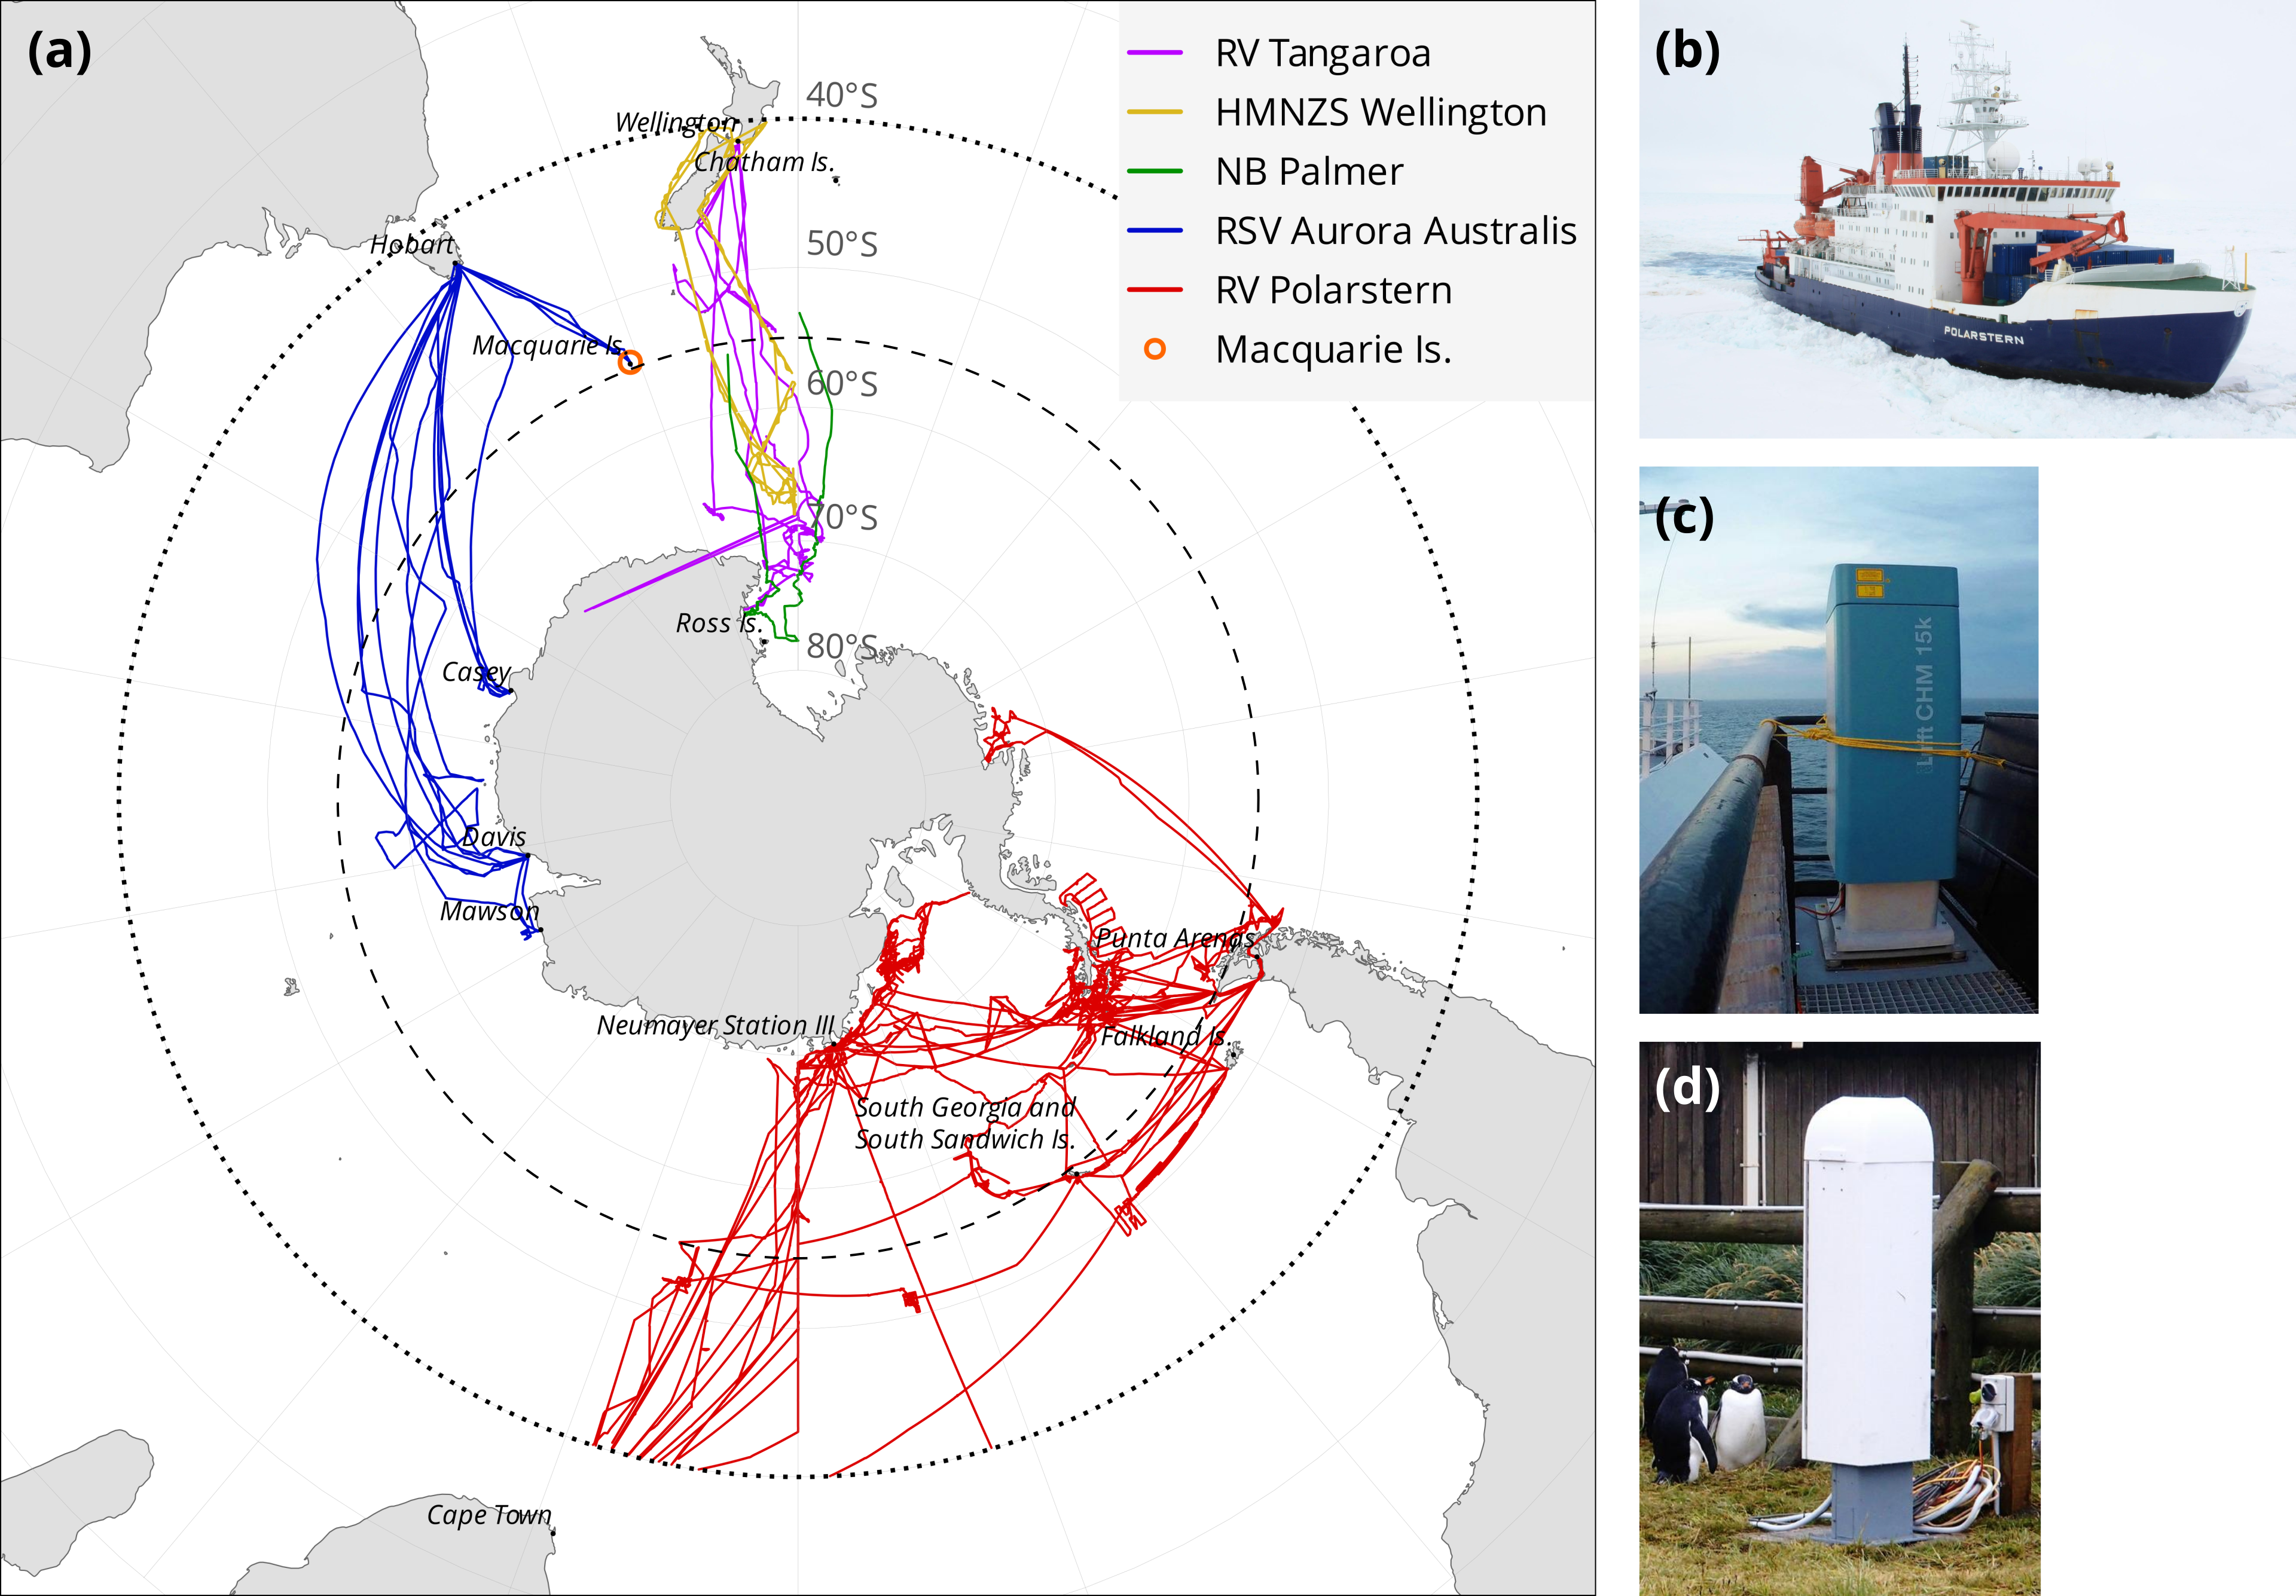
\includegraphics[width=\textwidth]{img/map_fig.pdf}
\caption{
\textbf{(a)} A map showing the tracks of 31 voyages of RV \emph{Polarstern},
RSV \emph{Aurora Australis}, RV \emph{Tangaroa}, RV \emph{Nathaniel B. Palmer},
and HMNZS \emph{Wellington} and one sub-Antarctic station (Macquarie Island)
analysed here. The tracks cover Antarctic sectors south of South America, the
Atlantic Ocean, Africa, Australia, and New Zealand in the years 2010--2021
(inclusive).  The dotted and dashed lines at 40°S and 55°S delineate the
Southern Ocean area of our analysis and its partitioning into two subsets,
respectively.  A photo of \textbf{(b)} RV \emph{Polarstern} (© Folke Mehrtens,
Alfred-Wegener-Institut), \textbf{(c)} Lufft CHM 15k installed on RV
\emph{Tangaroa} (© Peter Kuma, University of Canterbury), \textbf{(d)} Vaisala
CL51 (© Jeff Aquilina, Bureau of Meteorology).
}
\label{fig:map}
\end{figure}

\section{Methods}
\label{sec:methods}

\subsection{Voyage and station data}

Together, we analysed data from 31 voyages of RV \emph{Polarstern}, the resupply
vessel (RSV) \emph{Aurora Australis}, RV \emph{Tangaroa}, RV \emph{Nathaniel B.
Palmer}, Her Majesty's New Zealand Ship (HMNZS) \emph{Wellington} and one
sub-Antarctic station (Macquarie Island) in the SO south of 40°S between 2010
and 2021. Fig. \ref{fig:map} shows a map of the voyages, Table
\ref{tab:voyages} list the voyages, campaigns, and stations, and Table
\ref{tab:voyage-references} lists references where available. Altogether, the
voyages and station dataset comprised 2421 days of data south of 40°S, but the
availability of ceilometer data was slightly smaller due to gaps in
measurements.

Missing days in the ceilometer data were HMNZSW16 (7 days): 24--27 November, 10
December, 16--17 December 2016; Measurements of Aerosols, Radiation, and CloUds
over the Southern Ocean (MARCUS;  3 days): 8, 10 November, 10 December 2017;
Macquarie Island Cloud Radiation Experiment (MICRE; 9 days): 7--8, 29 June, 5,
16 July, 15 August, 17 October 2016, 11 February, 21 March 2017; TAN1502 (1
day): 24 January.

The data sources contained ceilometer observations captured by the Vaisala CL51
operating at a wavelength of 910 nm, the Vaisala CT25K operating at 905 nm, and
the Lufft CHM 15k operating at 1064 nm, described in detail below (Sections
\ref{sec:cl51} and \ref{sec:chm15k}). A ceilometer is a low-power near-infrared
vertically pointing lidar principally designed to  measure cloud base, but they
also measure the full vertical structure of clouds as long as the laser signal
is not attenuated by thick clouds, which can be used to infer additional
information such as a cloud mask and cloud occurrence by height.

Apart from lidar observations, radiosondes were launched on weather balloons at
regular synoptic times on the RV \emph{Polarstern}, MARCUS, NBP17024, TAN1702,
and TAN1802 voyages and campaigns, measuring pressure, temperature, relative
humidity, and the global navigation satellite system coordinates. Derived
thermodynamic (virtual potential temperature, lifting condensation level, etc.)
and dynamic physical quantities (wind speed and direction) for the measured
vertical profiles were calculated with rstool \citep{rstool}. Surface
meteorological quantities were measured continuously by an onboard automatic
weather station or individual instruments.

\begin{table}[p!]
\caption{
An overview of the analysed voyages, campaigns, and stations. Start, end, and
the number of days (UTC; inclusive) refer to the time period when the vessel
was south of 40°S.  Abbreviations: ceilometer (ceil.), Australia (AU), New
Zealand (NZ), South America (SA), Atlantic Ocean (AO), and Africa (AF). The
number of days is rounded to the nearest integer. CL51/31 indicates CL51
configured to emulate CL31.
}
\label{tab:voyages}
\small
\begin{tabular}{llllllr}
\textbf{Name} & \textbf{Vessel or station} & \textbf{Ceil.} & \textbf{Region} & \textbf{Start} & \textbf{End} & \textbf{Days}\\
\hline
AA15-16  & RSV \emph{Aurora Australis}   & CL51    & AU       & 2015-10-22 & 2016-02-22 & 124 \\
HMNZSW16 & HMNZS \emph{Wellington}       & CHM 15k & NZ       & 2016-11-23 & 2016-12-19 & 27 \\
MARCUS   & RSV \emph{Aurora Australis}   & CT25K   & AU       & 2017-10-29 & 2018-03-26 & 149 \\
MICRE    & Macquarie Is. station         & CT25K   & AU/NZ    & 2016-04-03 & 2018-03-14 & 710 \\
NBP1704  & RV \emph{Nathaniel B. Palmer} & CHM 15k & NZ       & 2017-04-14 & 2017-06-08 & 55 \\
PS77/2   & RV \emph{Polarstern}          & CL51    & SA/AO/AF & 2010-12-01 & 2011-02-04 & 65 \\
PS77/3   & RV \emph{Polarstern}          & CL51    & SA/AO/AF & 2011-02-07 & 2011-04-14 & 66 \\
PS79/2   & RV \emph{Polarstern}          & CL51    & SA/AO/AF & 2011-12-06 & 2012-01-02 & 27 \\
PS79/3   & RV \emph{Polarstern}          & CL51    & SA/AO/AF & 2012-01-10 & 2012-03-10 & 61 \\
PS79/4   & RV \emph{Polarstern}          & CL51    & SA/AO/AF & 2012-03-14 & 2012-04-08 & 26 \\
PS81/2   & RV \emph{Polarstern}          & CL51    & SA/AO/AF & 2012-12-02 & 2013-01-18 & 47 \\
PS81/3   & RV \emph{Polarstern}          & CL51    & SA/AO/AF & 2013-01-22 & 2013-03-17 & 55 \\
PS81/4   & RV \emph{Polarstern}          & CL51    & SA/AO/AF & 2013-03-18 & 2013-04-16 & 30 \\
PS81/5   & RV \emph{Polarstern}          & CL51    & SA/AO/AF & 2013-04-20 & 2013-05-23 & 33 \\
PS81/6   & RV \emph{Polarstern}          & CL51    & SA/AO/AF & 2013-06-10 & 2013-08-12 & 63 \\
PS81/7   & RV \emph{Polarstern}          & CL51    & SA/AO/AF & 2013-08-15 & 2013-10-14 & 60 \\
PS81/8   & RV \emph{Polarstern}          & CL51    & SA/AO/AF & 2013-11-12 & 2013-12-14 & 31 \\
PS81/9   & RV \emph{Polarstern}          & CL51    & SA/AO/AF & 2013-12-21 & 2014-03-02 & 71 \\
PS89     & RV \emph{Polarstern}          & CL51    & SA/AO/AF & 2014-12-05 & 2015-01-30 & 56 \\
PS96     & RV \emph{Polarstern}          & CL51    & SA/AO/AF & 2015-12-08 & 2016-02-14 & 68 \\
PS97     & RV \emph{Polarstern}          & CL51    & SA/AO/AF & 2016-02-15 & 2016-04-06 & 52 \\
PS103    & RV \emph{Polarstern}          & CL51    & SA/AO/AF & 2016-12-18 & 2017-02-02 & 46 \\
PS104    & RV \emph{Polarstern}          & CL51    & SA/AO/AF & 2017-02-08 & 2017-03-18 & 39 \\
PS111    & RV \emph{Polarstern}          & CL51    & SA/AO/AF & 2018-01-21 & 2018-03-14 & 52 \\
PS112    & RV \emph{Polarstern}          & CL51    & SA/AO/AF & 2018-03-18 & 2018-05-05 & 49 \\
PS117    & RV \emph{Polarstern}          & CL51    & SA/AO/AF & 2018-12-18 & 2019-02-07 & 51 \\
PS118    & RV \emph{Polarstern}          & CL51    & SA/AO/AF & 2019-02-18 & 2019-04-08 & 50 \\
PS123    & RV \emph{Polarstern}          & CL51    & SA/AO/AF & 2021-01-10 & 2021-01-31 & 21 \\
PS124    & RV \emph{Polarstern}          & CL51    & SA/AO/AF & 2021-02-03 & 2021-03-30 & 55 \\
TAN1502  & RV \emph{Tangaroa}            & CL51/31 & NZ       & 2015-01-20 & 2015-03-12 & 51 \\
TAN1702  & RV \emph{Tangaroa}            & CHM 15k & NZ       & 2017-03-09 & 2017-03-31 & 23 \\
TAN1802  & RV \emph{Tangaroa}            & CHM 15k & NZ       & 2018-02-07 & 2018-03-20 & 41 \\
\hline
\textbf{Total} &                         &         &          &            &            & \textbf{2421}\\
\end{tabular}
\normalsize
\end{table}

\begin{table}[t!]
\caption{Voyage, campaign and station publication references.}
\label{tab:voyage-references}
\small
\begin{tabular}{lp{14.5cm}}
\textbf{Name} & \textbf{References}\\
\hline
AA15-16  & \cite{klekociuk2020} \\
MARCUS   & \cite{mcfarquhar2021,xia2024,niu2024} \\
MICRE    & \cite{mcfarquhar2021} \\
NBP1704  & \cite{ackley2020} \\
PS77/2   & \cite{kniglanglo2011a,kniglanglo2011b,kniglanglo2011c,kniglanglo2014a,fahrbach2011} \\
PS77/3   & \cite{kniglanglo2011d,kniglanglo2011e,kniglanglo2012a,kniglanglo2014b,knust2011} \\
PS79/2   & \cite{kniglanglo2012b,kniglanglo2012c,kniglanglo2012d,kniglanglo2014c,kattner2012} \\
PS79/3   & \cite{kniglanglo2012e,kniglanglo2012f,kniglanglo2012g,kniglanglo2014d,wolfgladrow2012} \\
PS79/4   & \cite{kniglanglo2012h,kniglanglo2012i,kniglanglo2012j,kniglanglo2014e,lucassen2012} \\
PS81/2   & \cite{kniglanglo2013a,kniglanglo2013b,kniglanglo2013c,kniglanglo2014f,boebel2013} \\
PS81/3   & \cite{kniglanglo2013d,kniglanglo2013e,kniglanglo2013f,kniglanglo2014g,gutt2013} \\
PS81/4   & \cite{kniglanglo2013g,kniglanglo2013h,kniglanglo2013i,kniglanglo2014f,bohrmann2013} \\
PS81/5   & \cite{kniglanglo2013j,kniglanglo2013k,kniglanglo2013l,kniglanglo2014g,jokat2013} \\
PS81/6   & \cite{kniglanglo2013m,kniglanglo2013n,kniglanglo2013o,kniglanglo2014h,lemke2013} \\
PS81/7   & \cite{kniglanglo2013p,kniglanglo2013q,kniglanglo2014i,kniglanglo2016a,meyer2013} \\
PS81/8   & \cite{kniglanglo2013r,kniglanglo2014j,kniglanglo2014k,kniglanglo2014l,schlindwein2014} \\
PS81/9   & \cite{kniglanglo2014m,kniglanglo2014n,kniglanglo2014o,kniglanglo2014p,knust2014} \\
PS89     & \cite{kniglanglo2015a,kniglanglo2015b,kniglanglo2015c,kniglanglo2015d,boebel2016}\\
PS96     & \cite{kniglanglo2016b,kniglanglo2016c,kniglanglo2016d,kniglanglo2016e,schrder2017} \\
PS97     & \cite{kniglanglo2016f,kniglanglo2016g,kniglanglo2016h,kniglanglo2016i,lamy2017} \\
PS103    & \cite{kniglanglo2017a,kniglanglo2017b,kniglanglo2017c,kniglanglo2017d,boebel2018} \\
PS104    & \cite{kniglanglo2017e,kniglanglo2017f,kniglanglo2017g,gohl2018,schmithsen2021a} \\
PS111    & \cite{schmithsen2019a,schmithsen2020a,schmithsen2021b,schmithsen2021c,schrder2018} \\
PS112    & \cite{schmithsen2019b,schmithsen2020b,schmithsen2021d,schmithsen2021e,meyer2018} \\
PS117    & \cite{schmithsen2019c,schmithsen2020c,schmithsen2021f,schmithsen2021g,boebel2019} \\
PS118    & \cite{schmithsen2019d,schmithsen2020d,schmithsen2021h,schmithsen2021i,dorschel2019} \\
PS123    & \cite{schmithsen2021j,schmithsen2021m,schmithsen2021n,schmithsen2021k,hoppmann2023} \\
PS124    & \cite{schmithsen2021o,schmithsen2021q,schmithsen2021p,hoppmann2023} \\
TAN1802  & \cite{kremser2020,kremser2021} \\
\end{tabular}
\end{table}

\subsection{Vaisala CL51 and CT25K}
\label{sec:cl51}

The Vaisala CL51 (photo in Fig. \ref{fig:map}d) and CT25K are ceilometers
operating at a near-infrared wavelength of 910 nm and 905 nm, respectively.
The CL51 can also be configured to emulate the Vaisala CL31. The maximum range is
15.4 km (CL51), 7.7 km (CL31 emulation mode with 5 m vertical resolution), and
7.5 km (CT25K). The vertical resolution is 10 m (5 m configurable) in CL51 and
30 m in CT25K observations. The sampling (temporal) resolution is configurable, and in our
datasets is approximately 6 s for CL51 on AA15‐16, 16 s for CT25K on MARCUS and
MICRE, 36 s for CL51 on RV \emph{Polarstern}, and about 2.37 s for CL51 with
CL31 emulation on TAN1502. The wavelength of 910 nm is affected by water vapour
absorption of about 20\% in the mid-latitudes \citep{wiegner2015,wiegner2019},
but we do not expect this to be a significant issue as explained in
\cite{kuma2021}.  The instrument data files containing raw uncalibrated
backscatter were first converted to Network Common Data Form (NetCDF) with
cl2nc (\url{https://github.com/peterkuma/cl2nc}) and then processed with the
ALCF (Section \ref{sec:alcf}) to produce absolutely calibrated attenuated
volume backscattering coefficient (AVBC), cloud mask, cloud occurrence by
height, and the total cloud fraction. Because the CT25K uses a very similar
wavelength to CL51, equivalent calculations as for CL51 were done assuming a
wavelength of 910 nm. The Vaisala CL51 and CT25K instruments were used on most
of the voyages and stations analysed here. Fig.  \ref{fig:example}a shows an
example of AVBC derived from the CL51 instrument data.

\begin{figure}[b!]
\centering
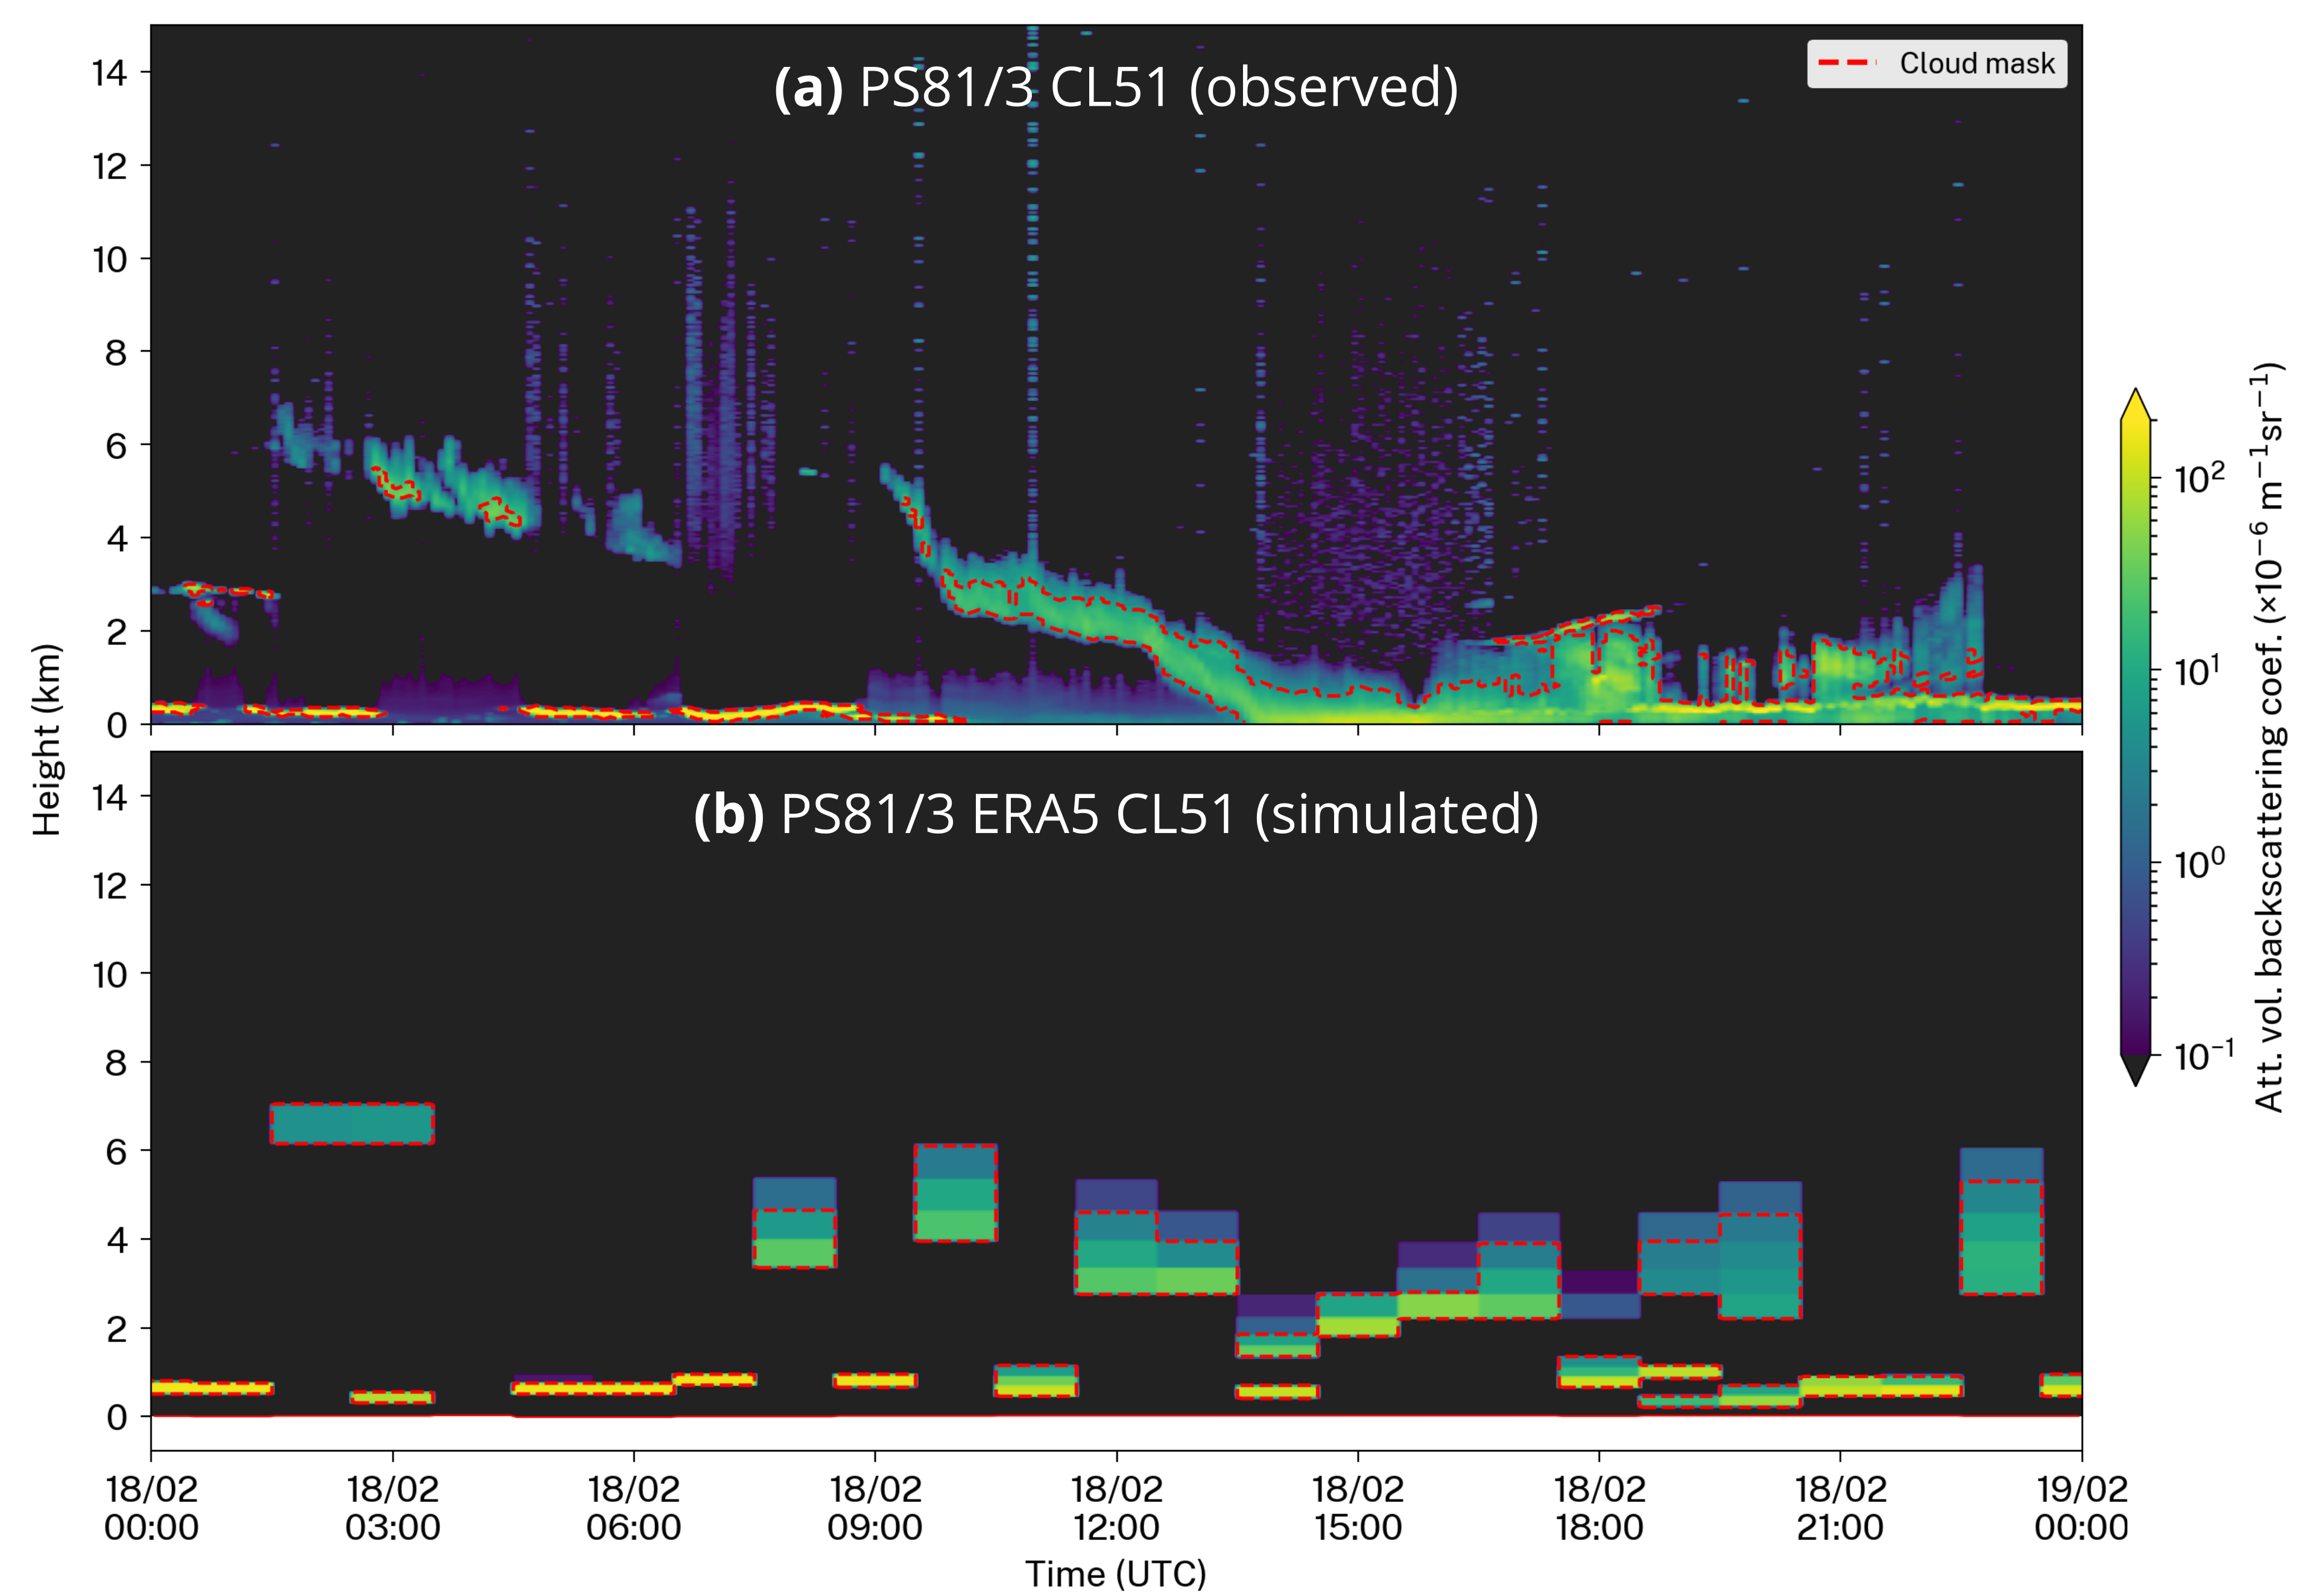
\includegraphics[width=\textwidth]{img/example.png}
\caption{
An example of attenuated volume backscattering coefficient (AVBC) \textbf{(a)}
measured by CL51 during 24 hours on the PS81/3 voyage and \textbf{(b)} an
equivalent AVBC simulated with the ALCF from ERA5 data during the same time
period. The red line identifies the cloud mask determined by the ALCF.
}
\label{fig:example}
\end{figure}

\subsection{Lufft CHM 15k}
\label{sec:chm15k}

The Lufft CHM 15k (photo in Fig. \ref{fig:map}c) is a ceilometer operating at a
near-infrared wavelength of 1064 nm. The maximum range is 15.4 km, the vertical
resolution is 5 m in the near range (up to 150 m) and 15 m above, the sampling
(temporal) resolution is 2 s, and the number of vertical levels is 1024.
NetCDF files containing uncalibrated backscatter produced by the instrument
were processed with the ALCF (Section \ref{sec:alcf}) to again produce AVBC, cloud
mask, cloud occurrence by height, and the total cloud fraction. The CHM 15k was
used on four voyages (HMNZSW16, TAN1702, TAN1802, and NBP1704).

\subsection{ALCF}
\label{sec:alcf}

The Automatic Lidar and Ceilometer Framework (ALCF) is a ground-based lidar
simulator and a tool for processing observed lidar data, supporting various
instruments and models \citep{kuma2021}. It performs radiative transfer
calculations to derive equivalent lidar AVBC in an atmospheric model, which can
then be compared with observed AVBC. For this purpose, it takes the cloud fraction, liquid and ice mass mixing ratio, temperature, and
pressure model fields as an input and is run offline (on the model output rather than
inside the model code). The lidar simulator in the ALCF is based on the
instrument simulator Cloud Feedback Model Intercomparison Project (CFMIP)
Observation Simulator Package (COSP) \citep{bodas-salcedo2011}.  After AVBC is
calculated, a cloud mask, cloud occurrence by height, and the total cloud
fraction are determined. The ALCF has been used by several research teams for
model and reanalysis evaluation
\citep{kuma2020,kremser2021,guyot2022,pei2023,whitehead2023,mcdonald2024}.

Absolute calibration of the observed backscatter was performed by comparing the
measured clear-sky molecular backscatter statistically with simulated clear-sky
molecular backscatter. AVBC was resampled to 5 min temporal resolution and 50 m
vertical resolution to increase signal-to-noise ratio while having enough
resolution to detect small-scale cloud variability. The noise standard
deviation was calculated from AVBC at the highest range, where no clouds are
expected.  A cloud mask was calculated from AVBC using a fixed threshold of
$\mathrm{2\times 10^{-6} m^{-1}sr^{-1}}$ after subtracting 5 standard
deviations of range-scaled noise. Fig. \ref{fig:example}b shows an example of
simulated Vaisala CL51 backscatter from ERA5 data, corresponding to a day of
measurements by the instrument on the PS81/3 voyage.

\subsection{ICON}

A coupled (atmosphere--ocean) GSRM version of the ICON model is in development
at the nextGEMS project \citep{hohenegger2023}. ICON is an exceptionally
versatile model, allowing for simulations ranging from coarse-resolution ESM
simulations, GSRM simulations, limited area model simulations, to large eddy
simulations (LES), for both weather prediction and climate projections. ICON
uses the atmospheric component ICON-A \citep{giorgetta2018}, whose physics is
derived from ECHAM6 \citep{stevens2013}, and the ocean component ICON-O
\citep{korn2022}. Earlier runs of the GSRM ICON from DYAMOND were evaluated by
\cite{mauritsen2022}.

Here, we use a free-running (i.e., \emph{not} nudged or using prescribed SST)
coupled GSRM simulation made for the purpose of climate projection.  nextGEMS
has so far produced four cycles of model runs. We used a Cycle 3 run
\emph{ngc3028} produced in 2023 \citep{nextgems2023a,nextgems2023b} for a model
time period of 20 January 2020 to 22 July 2025, of which we analysed the period 2021--2024 (inclusive). While a Cycle 4 run was available, we could not
use it due to a lack of availability of the necessary variables. The horizontal
resolution of ngc3028 is about 5 km.  The model output is available on 90
vertical levels and 3-hourly instantaneous temporal resolution.  Unlike current
general circulation models (GCMs), the storm-resolving version of ICON does not
use convective and cloud parameterization but relies on explicit simulation of
convection and clouds on the model grid. While this makes the code development
simpler without having to rely on uncertain parameterizations, it can miss
smaller-scale clouds below the grid resolution.  Turbulence and cloud
microphysics are still parameterized in this model.

Because the model is free-running, weather and climate oscillations (such as
the El Niño--Southern Oscillation) are not expected to be equivalent to reality
at the same time and place. To compare with the observations collected in
different years (2010--2021, inclusive), we compared the model output with
observations at the same time of year and geographical location, as determined
for each data point such as a lidar profile or a radiosonde launch.

\subsection{MERRA-2}

The Modern-Era Retrospective analysis for Research and Applications, Version 2
(MERRA-2) is a reanalysis produced by the Global Modeling and Assimilation
Office at the NASA Goddard Space Flight Center \citep{gelaro2017}.  It uses
version 5.12.4 of the Goddard Earth Observing System (GEOS) atmospheric model
\citep{rienecker2008,molod2015}. The reanalysis output analysed here is
available at a spatial resolution of 0.5° of latitude and 0.625° of longitude,
which is about 56 km in the North--South direction and 35 km in the East--West
direction at 60°S. The number of vertical model levels is 72. Here, we use the
following products: 1-hourly instantaneous 2D single-level diagnostics
(M2I1NXASM) for 2-m temperature and humidity; 3-hourly instantaneous 3D
assimilated meteorological fields (M2I3NVASM) for cloud quantities, pressure,
and temperature; 1-hourly average 2D surface flux diagnostics (M2T1NXFLX) for
precipitation; and 1-hourly average 2D radiation diagnostics
(M2T1NXRAD) for radiation quantities \citep{merra2}.

\subsection{ERA5}

ERA5 \citep{era5} is a reanalysis produced by the ECMWF.  It is based on a
numerical weather prediction model IFS version CY41R2.  The horizontal
resolution is 0.25° in latitude and longitude, which is about 28 km in the
North--South direction and 14 km in the East--West direction at 60°S.
Internally, the model uses 137 vertical levels. Here, we use output at 1-hourly
instantaneous time intervals, except for radiation quantities, which are
accumulations (from these we calculate daily means).  Vertically resolved
quantities are made available on 37 pressure levels.

\subsection{CERES}

TOA radiation quantities are taken from the CERES instruments on board the
Terra and Aqua satellites \citep{wielicki1996,loeb2018}. In our analysis we
used the adjusted all sky SW and LW upwelling fluxes at TOA from the synoptic
TOA and surface fluxes and clouds 1 degree daily edition 4A product
(CER\_SYN1deg-Day\_Terra-Aqua-MODIS\_Edition4A)
\citep{doelling2013,doelling2016}.

Radiation calculations presented in the results (Section \ref{sec:results})
were done in such a way that they always represent averages of daily means.
This was done in order to be consistent with the CERES SYN1deg data, which are
available as daily means. Therefore, every instantaneous profile in the
simulated lidar data was assigned a daily mean radiation value corresponding to
the day (in the Coordinated Universal Time; UTC). In turn, the average
radiation during the entire voyage or station observation period were
calculated as the average of the profile values. In the observed lidar data,
the daily mean radiation value was taken from the spatially and temporally
co-located CERES SYN1deg data of the day (in UTC). The voyage or station
average was calculated in the same way.

\begin{figure}[b!]
\centering
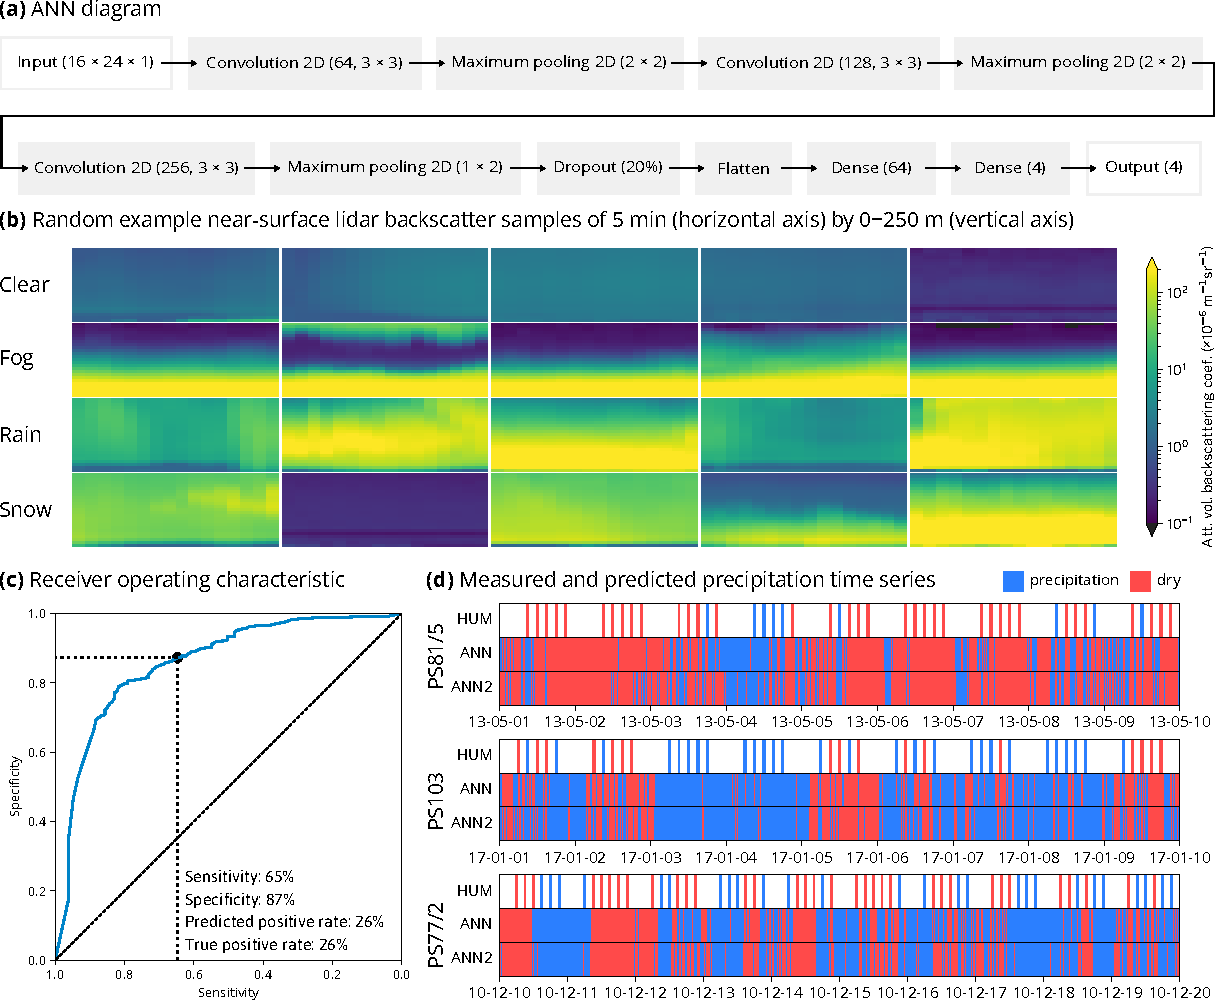
\includegraphics[width=\textwidth]{img/ann.pdf}
\caption{
Artificial neural network (ANN) for prediction of precipitation in lidar
backscatter. \textbf{(a)} Diagram showing the TensorFlow structure of the ANN,
\textbf{(b)} randomly selected example samples of near-surface backscatter in
four categories (clear, fog, rain, and snow), as determined by coincident
human-performed weather observations, \textbf{(c)} receiver operating
characteristic diagram of the ANN, \textbf{(d)} examples of 10-day time series
of human-observed (`HUM') and predicted precipitation based on an ANN trained
on all voyages (`ANN') and all voyages except for the shown voyage (`ANN2')
during three randomly selected voyages with the available data. Here, by
`randomly selected' we mean selected from the top of a permutation generated by
a pseudo-random number generator to prevent authors' bias in the selection.
}
\label{fig:ann}
\end{figure}

\subsection{Precipitation identification using machine learning}
\label{sec:ann}

Precipitation can cause strong enough lidar backscattering to be recognised as
clouds by the threshold-based cloud detection method used in the ALCF. This is
undesirable if equivalent precipitation backscatter is not included in the
simulated lidar profiles. It was not possible to include precipitation
simulation in the ALCF due to the absence of required fields in the ICON model
output and the reanalysis data (the liquid and ice precipitation mass mixing
ratios). The required radiation calculations for precipitation are also
currently not implemented in the ALCF, even though this is a planned feature.
In order to achieve a fair comparison of observations with models, one should
exclude observed and simulated lidar profiles with precipitation either
manually or using an automated method. It is relatively difficult to
distinguish precipitation backscatter from cloud backscatter in lidar
observations, especially when only one wavelength channel and no polarised
channel are available. In models, the same can be accomplished relatively
easily by excluding profiles exceeding a certain amount of surface
precipitation flux. In the observations, using precipitation flux measurements
from rain gauges can be very unreliable on ships due to ship movement,
turbulence caused by nearby ship structures, and sea spray. Our analysis of
rain gauge data from the RV \emph{Tangaroa} showed large discrepancies between
the rain gauge time series and human-performed synoptic observations, as well
as large inconsistencies in the rain gauge time series. Human-performed
observations of precipitation presence or absence are expected to be reliable
but only cover a limited set of time instants. Therefore, it was desirable to
implement a method of detecting precipitation from observed backscatter
profiles alone.

On the RV \emph{Polarstern} voyages, regular human-performed synoptic
observations were available and included precipitation presence or absence and
type. We used this dataset to train a convolutional artificial neural network
(ANN) to recognise profiles with precipitation from lidar backscatter (Fig.
\ref{fig:ann}a), implemented in the TensorFlow ANN framework
\citep{tensorflow}. Samples of short time intervals (10 min) of near-surface
lidar backscatter (0–250 m) were classified as clear, rain, snow, and fog,
using the synoptic observations as a training dataset (Fig.  \ref{fig:ann}b).
From these, a binary, mutually exclusive classification of profiles as
precipitating (rain or snow) or dry (clear or fog) was derived.  For detecting
model and reanalysis precipitation, we used a fixed threshold for surface
precipitation flux of 0.1 mm h$^{-1}$ (the ANN was not used).

The ANN achieved 65\% sensitivity and 87\% specificity when the true positive
rate (26\%) was made to match observations. The receiver operating
characteristic curve is shown in Fig. \ref{fig:ann}c. We considered these rates
satisfactory for the purpose of filtering precipitation profiles. Fig.
\ref{fig:ann}d shows examples of the predicted precipitation compared to
human-performed observations.

\begin{figure}[b!]
\centering
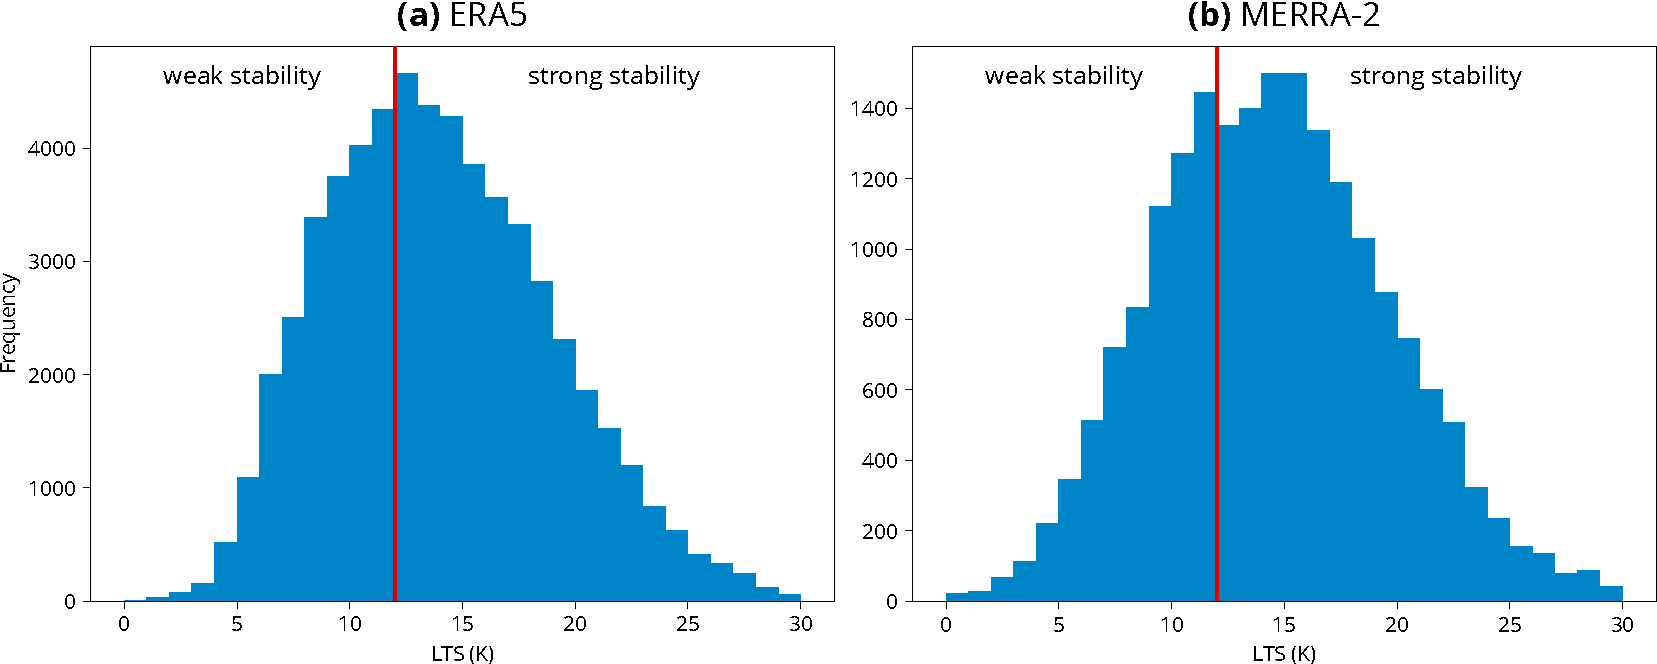
\includegraphics[width=\textwidth]{img/lts_dist.pdf}
\caption{
Lower tropospheric stability (LTS) distribution in \textbf{(a)} ERA5 and
\textbf{(b)} MERRA-2 calculated for the 31 voyage tracks and one station from
the highest instantaneous temporal resolution data available. Shown is also the
chosen dividing threshold of 12 K for relatively stable and unstable
conditions.
}
\label{fig:lts}
\end{figure}

\subsection{Partitioning by cyclonic activity and stability}
\label{sec:cyclone-stability}

We partitioned our data into two mutually exclusive subsets by cyclonic
activity. For this purpose, we used a cyclone tracking algorithm to identify
extratropical and polar cyclones (ECs and PCs) over the SO in the reanalysis
and ICON data. We used the open source cyclone tracking package CyTRACK
\citep{perez-alarcon2024}.  Generally, what constitutes an EC is considered
relatively arbitrary due to the very large variability of ECs \citep{neu2013}.
We used the mean sea level pressure field and horizontal wind speed fields as
input to the CyTRACK algorithm. The algorithm uses pressure and wind speed
thresholds as well as tracking across time steps to identify cyclone centres
and radii. With this information, we could classify geographical areas as
either cyclonic or non-cyclonic. Due to a relatively small total area covered,
we chose a circle of a double radius (relative to one identified by CyTRACK)
centred at the cyclone centre as a cyclonic area for every time step and
cyclone. All other areas were identified as non-cyclonic. For identifying
cyclones in the observations and the reanalyses, ERA5 pressure and wind fields
were used as the input to CyTRACK.  This is justified by the fact that the
large-scale pressure and wind fields in ERA5 are likely sufficiently close to
reality. For identifying cyclones in ICON, its own pressure and wind fields
were used as the input to CyTRACK, because the model is free-running, and thus
the pressure and wind fields are different from reality.

In addition to the above, we partitioned our data into two mutually exclusive
subsets by stability. We determined this by calculating lower tropospheric
stability (LTS) as the difference between the potential temperature at 700 hPa
and the surface.  Based on a histogram of LTS in ERA5 and MERRA-2 calculated at
all voyage tracks and stations (Fig.  \ref{fig:lts}), we determined a dividing
threshold of 12 K for relatively unstable (< 12 K) and relatively stable (>= 12
K) conditions.

\section{Results}
\label{sec:results}

\begin{figure}[p!]
\centering
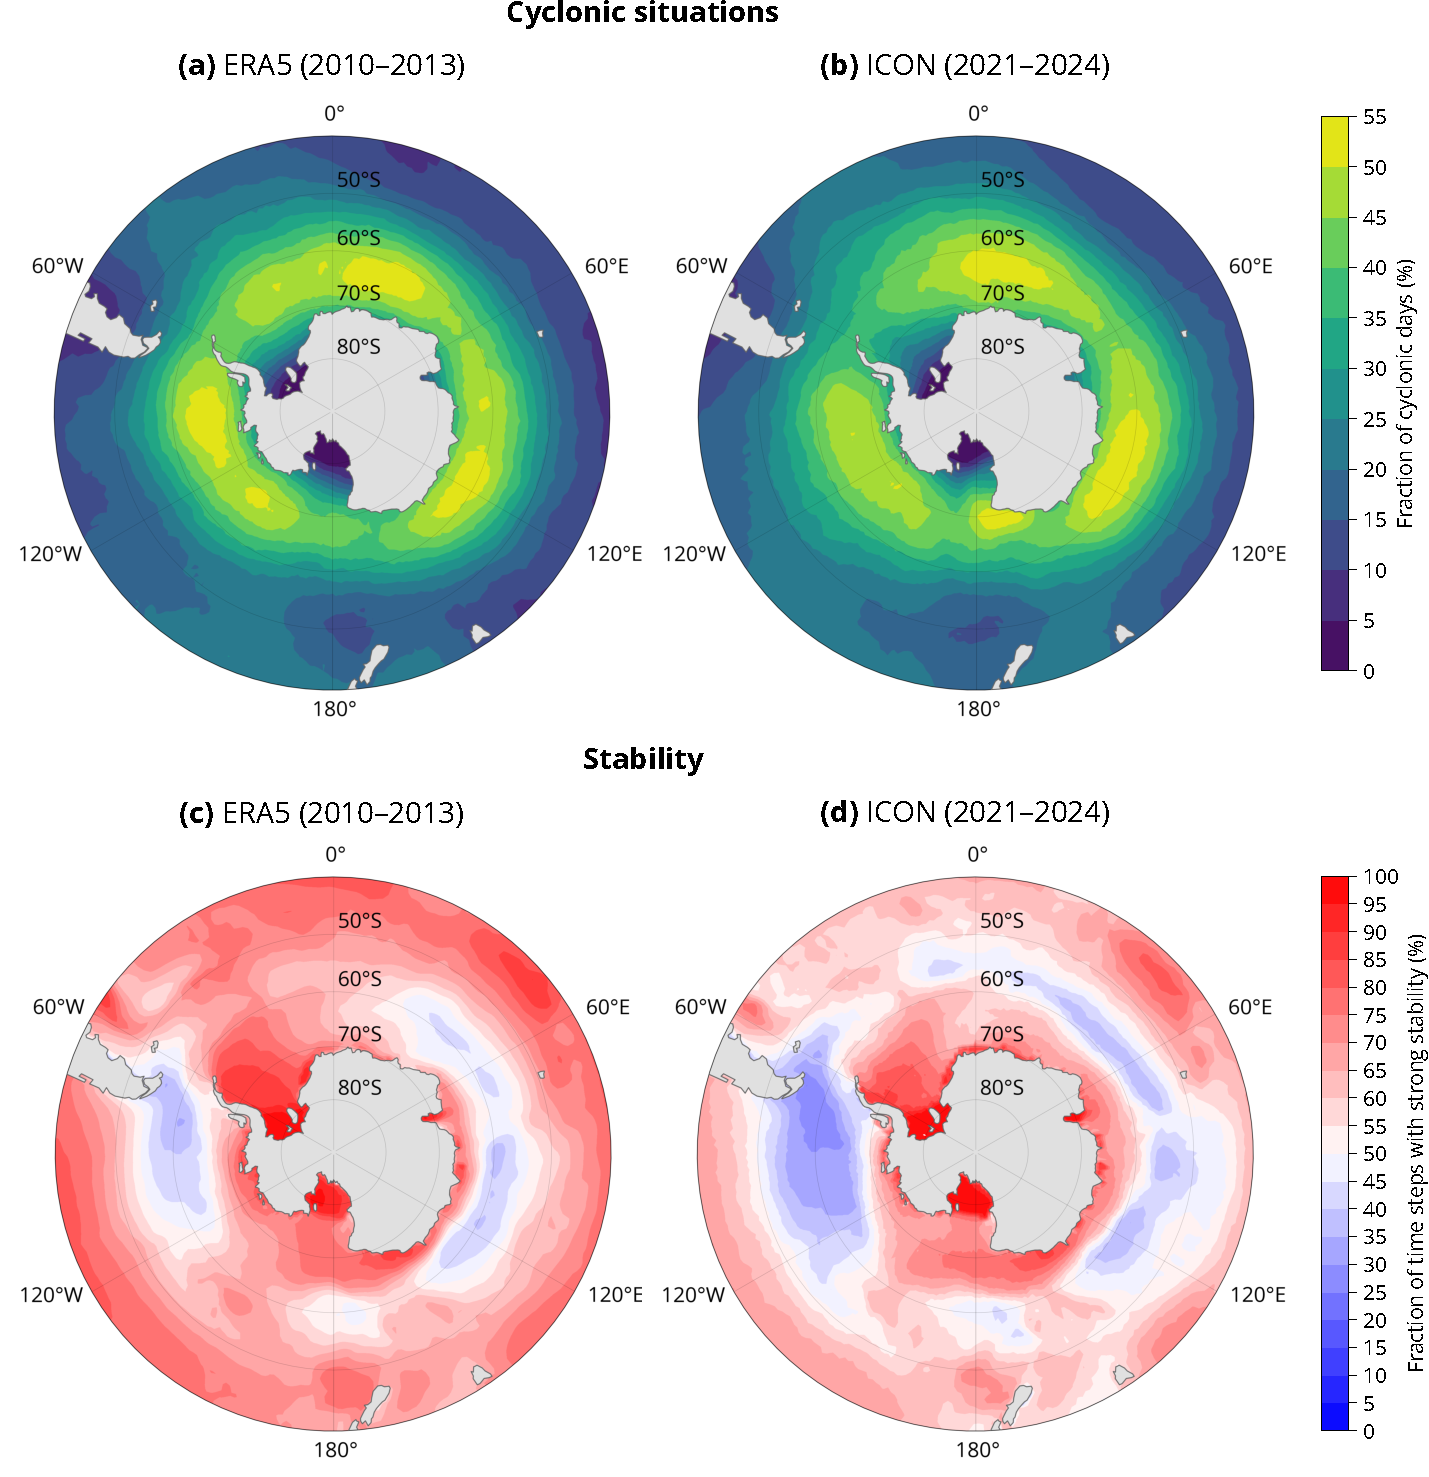
\includegraphics[width=\textwidth]{img/cyc_stab_dist.pdf}
\caption{
Geographical distribution of \textbf{(a, b)} cyclonic days and \textbf{(b, d)}
relatively stable (LTS > 12 K) time steps in \textbf{(a, c)} ERA5 in years
2010--2013 (inclusive) and \textbf{(b, d)} ICON in model years 2021--2023 (free
running). Cyclonic days are expressed as a fraction of the number of days with
cyclonic activity, defined as grid points located within a double radius of any
cyclone on a given day (UTC), as identified by CyTRACK.
}
\label{fig:cyclone-stability}
\end{figure}

\subsection{Cyclonic activity and stability}

Here, we briefly describe the results of the cyclonic activity and stability
distribution, which is relevant for the subsequent analysis, because these
conditions are used for subsetting our dataset. Fig.
\ref{fig:cyclone-stability}a, b show a geographical distribution of the fraction
of cyclonic days as determined by the cyclone tracking algorithm applied on the
ERA5 reanalysis and ICON data (Section \ref{sec:cyclone-stability}). As
expected, the strongest cyclonic activity is in the high-latitude SO zone, and
it is relatively zonally symmetric at all latitudes.  While both reanalysis and
the model agree relatively well, differences in the strength of the local
extremes of occurrence are notable, especially over the Amundsen Sea, which is
more cyclonic in the reanalysis, and around Cape Adare, which is more cyclonic
in ICON. These differences might, however, stem from the relatively short time
periods of comparison (4 years) and the fact that the model is free-running.

Fig. \ref{fig:cyclone-stability}c, d show a geographical distribution of the
relatively stable and unstable conditions as determined by the LTS (Section
\ref{sec:cyclone-stability}). Relatively unstable conditions are prevalent
in the middle SO (50--65°S), which might be explained by the relatively cold
near-surface air overlying the relatively warm sea surface. Relatively
stable conditions are prevalent elsewhere over the SO. The distribution is also
less zonally symmetric than the cyclonic activity.  In the high-latitude SO,
the presence of sea ice might have substantial stabilising effect
\citep{knight2024}. The ERA5 reanalysis is also substantially more stable than
ICON across the whole region.

\begin{figure}[p!]
\centerline{
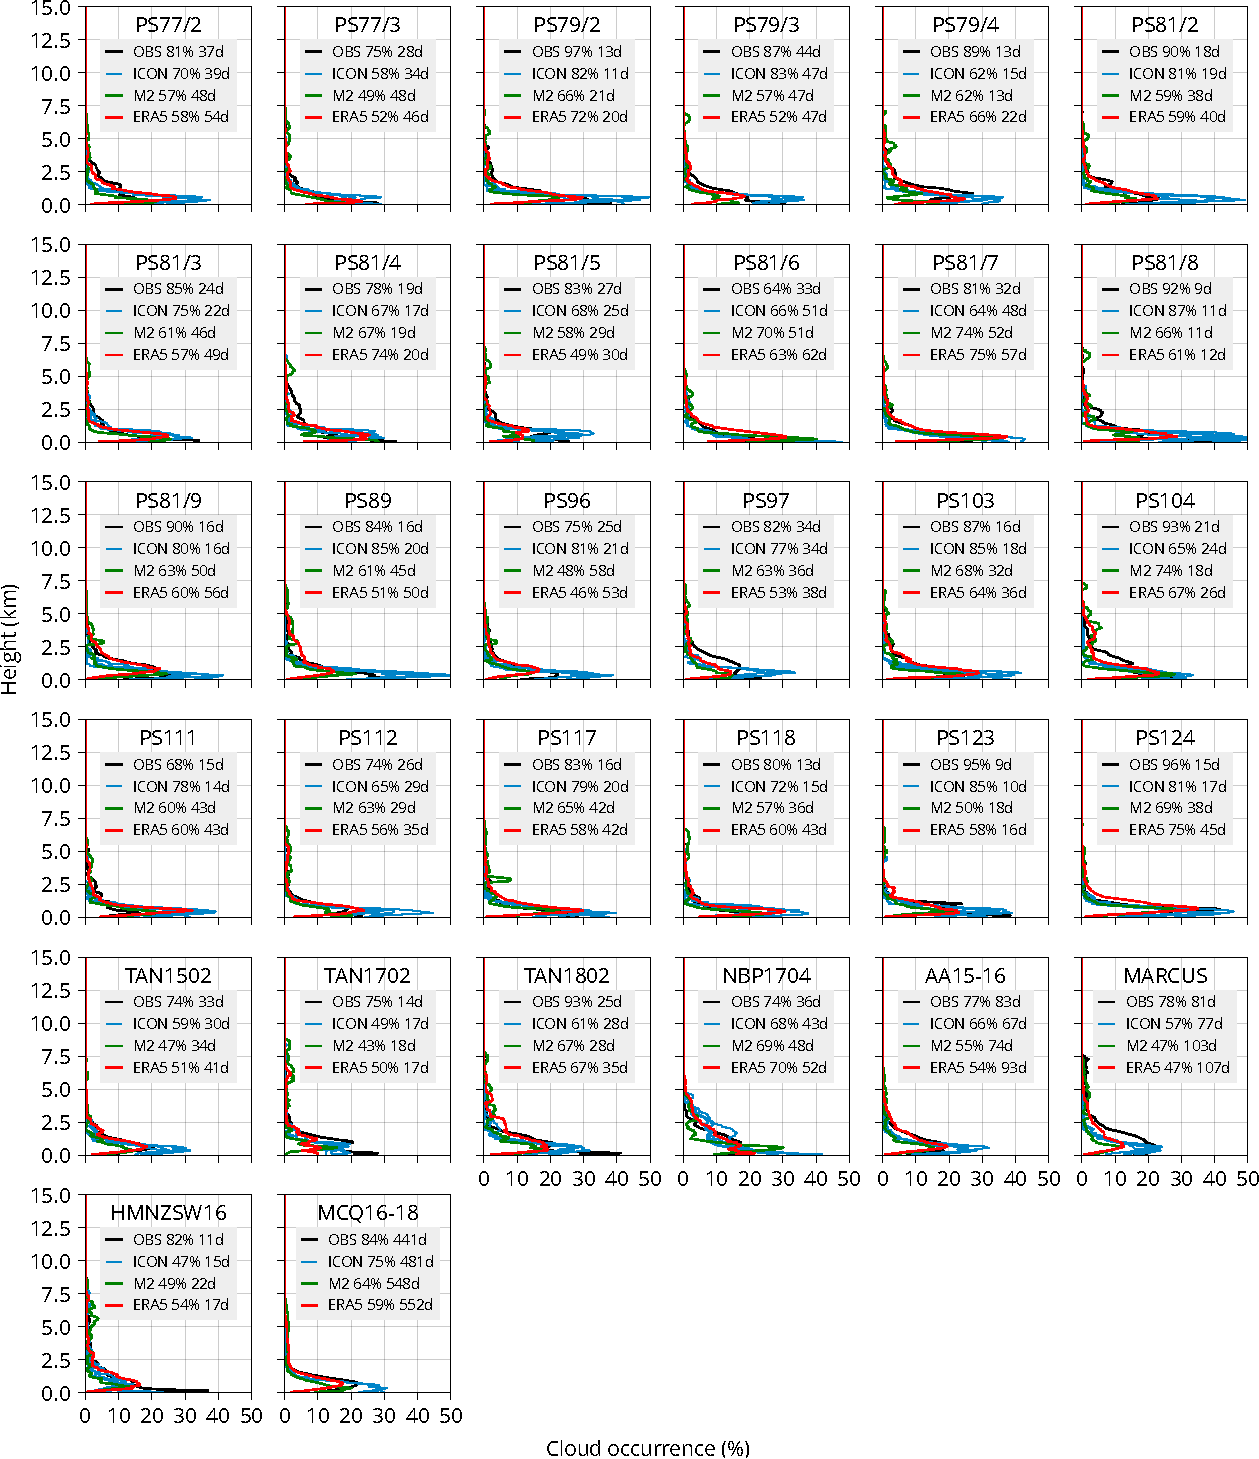
\includegraphics[width=1.06\textwidth]{img/cloud_occurrence_panel.pdf}
}
\caption{Cloud occurrence by height for the 31 voyages and one sub-Antarctic
station (MICRE) in observations (OBS) and simulated by the ALCF from the
ICON model, MERRA‐2 (M2), and ERA5 reanalysis data. The numbers in the legend
indicate the total cloud fraction and the number of days of data.}
\label{fig:cloud-occurrence-panel}
\end{figure}

\subsection{Cloud occurrence by height}
\label{sec:cloud-occurrence}

We used the ALCF to derive cloud occurrence by height and the total cloud
fraction from observations, ICON, ERA5 and MERRA-2 (Fig.
\ref{fig:cloud-occurrence-panel}). In addition, we aggregated the data sources
(voyages and stations) by calculating the averages and percentiles of all
individual profiles, presented in Fig. \ref{fig:cloud-occurrence}. The analysis
shows that the total cloud fraction (determined as the fraction of profiles
with clouds at any height in the lidar cloud mask) is underestimated in ICON
and the reanalyses by about 10\% and 20\%, respectively. When analysed by
height, ICON overestimates cloud occurrence below 1 km and underestimates it
above, MERRA-2 underestimates cloud occurrence at all heights, especially near
the surface, and ERA5 simulates cloud occurrence relatively well above 1 km,
but strongly underestimates it near the surface.  We note that fog or
near-surface clouds are strongly lacking in the reanalyses (fog and clouds are
both included in the cloud occurrence).  As shown in Fig.
\ref{fig:cloud-occurrence-panel}, the biases are relatively consistent across
the data sources and longitudes. We conclude that the ICON results are overall
better matching the observations than the reanalyses in this metric.

In the general case (Fig. \ref{fig:cloud-occurrence}a), the observations show
cloud occurrence peaking at the surface, whereas models show a higher peak (at
about 500 m). The models underestimate the total cloud fraction by 10--20\% and
show a strong drop in cloud occurrence near the surface, but this is not
supported by the observations. ICON and ERA5 overestimate cloud occurrence at
the peak (between 0--1 km). Above 1 km, ICON and MERRA-2 underestimate cloud
occurrence, but ERA5 is very accurate. The exaggerated peak in models is partly
supported by the lifting condensation level (LCL) distribution, which peaks
higher in the models than in the observations (at the surface), although this
is not very pronounced.

When subsetted by low- and high-latitude zones (Fig.
\ref{fig:cloud-occurrence}b, c), we see that the low-latitude SO zone shows
a stronger peak of cloud occurrence near the surface than the high-latitude SO
zone, and this could be because higher latitudes have more unstable atmospheric
profiles. The low- and high-latitude SO zones show similar biases in models as
in the general case, but ERA5 does not overestimate the peak in the
low-latitude SO zone (near-surface cloud occurrence is still strongly
underestimated).

When subsetted by cyclonic and non-cyclonic situations (Fig.
\ref{fig:cloud-occurrence}d, e), we see that the cyclonic situations have a
larger amount of observed cloudiness, including the peak and total cloud
fraction. In these situations, the models are doing a relatively good job of
getting the vertical profile of cloud occurrence right, but still tend to
underestimate cloud occurrence above 1 km and near the surface. Non-cyclonic
situations are similar to the general case.

When subsetted by relatively stable and unstable conditions (Fig.
\ref{fig:cloud-occurrence}f, g), as defined in Section
\ref{sec:cyclone-stability}, we see that in relatively stable
situations cloud occurrence peaks strongly at the surface in observations,
compared to relatively unstable situations, where the peak is more obtuse
and spread across the altitudes of 0--1 km.  In relatively stable
situations, the models are doing a fairly good job, but overestimate cloud
occurrence at the peak below 1 km; above 1 km, they show similar biases as in
the general case.  In relatively unstable situations, the bias in ICON is
very pronounced, with a much stronger peak at about 500 m, ERA5 is
underestimating cloud occurrence below 1 km (especially near the surface), and
MERRA-2 is underestimating it even more strongly.

In all situations, even when the models overestimate cloud occurrence at some
altitudes, they always substantially underestimate the total cloud fraction.
ICON can be generally characterised as substantially overestimating cloud
occurrence below 1 km and underestimating above, underestimating the total
cloud fraction, and showing greatest biases in relatively unstable and
non-cyclonic conditions. It also shows a peak of cloud occurrence at higher
altitude than observations (500 m vs. near the surface), and correspondingly,
its LCL tends to be also higher. MERRA-2 can be generally characterised as
underestimating cloud occurrence at nearly all altitudes as well as the total
cloud fraction, but mostly above and below 500 m (the peak at 500 m is
well-represented). It struggles the most in the low-latitude SO zone and in the
relatively unstable situations. ERA5 can be generally characterised as
representing cloud occurrence correctly above about 1--1.5 km, overestimating
below, but underestimating near-surface cloud occurrence (0--500 m). The total
cloud fraction is strongly underestimated in all situations. It has a tendency
towards underestimation in the low-latitude SO zone and relatively unstable
situations; conversely, overestimating in the high-latitude SO zone and the
relatively stable conditions.

\begin{figure}[p!]
\centering
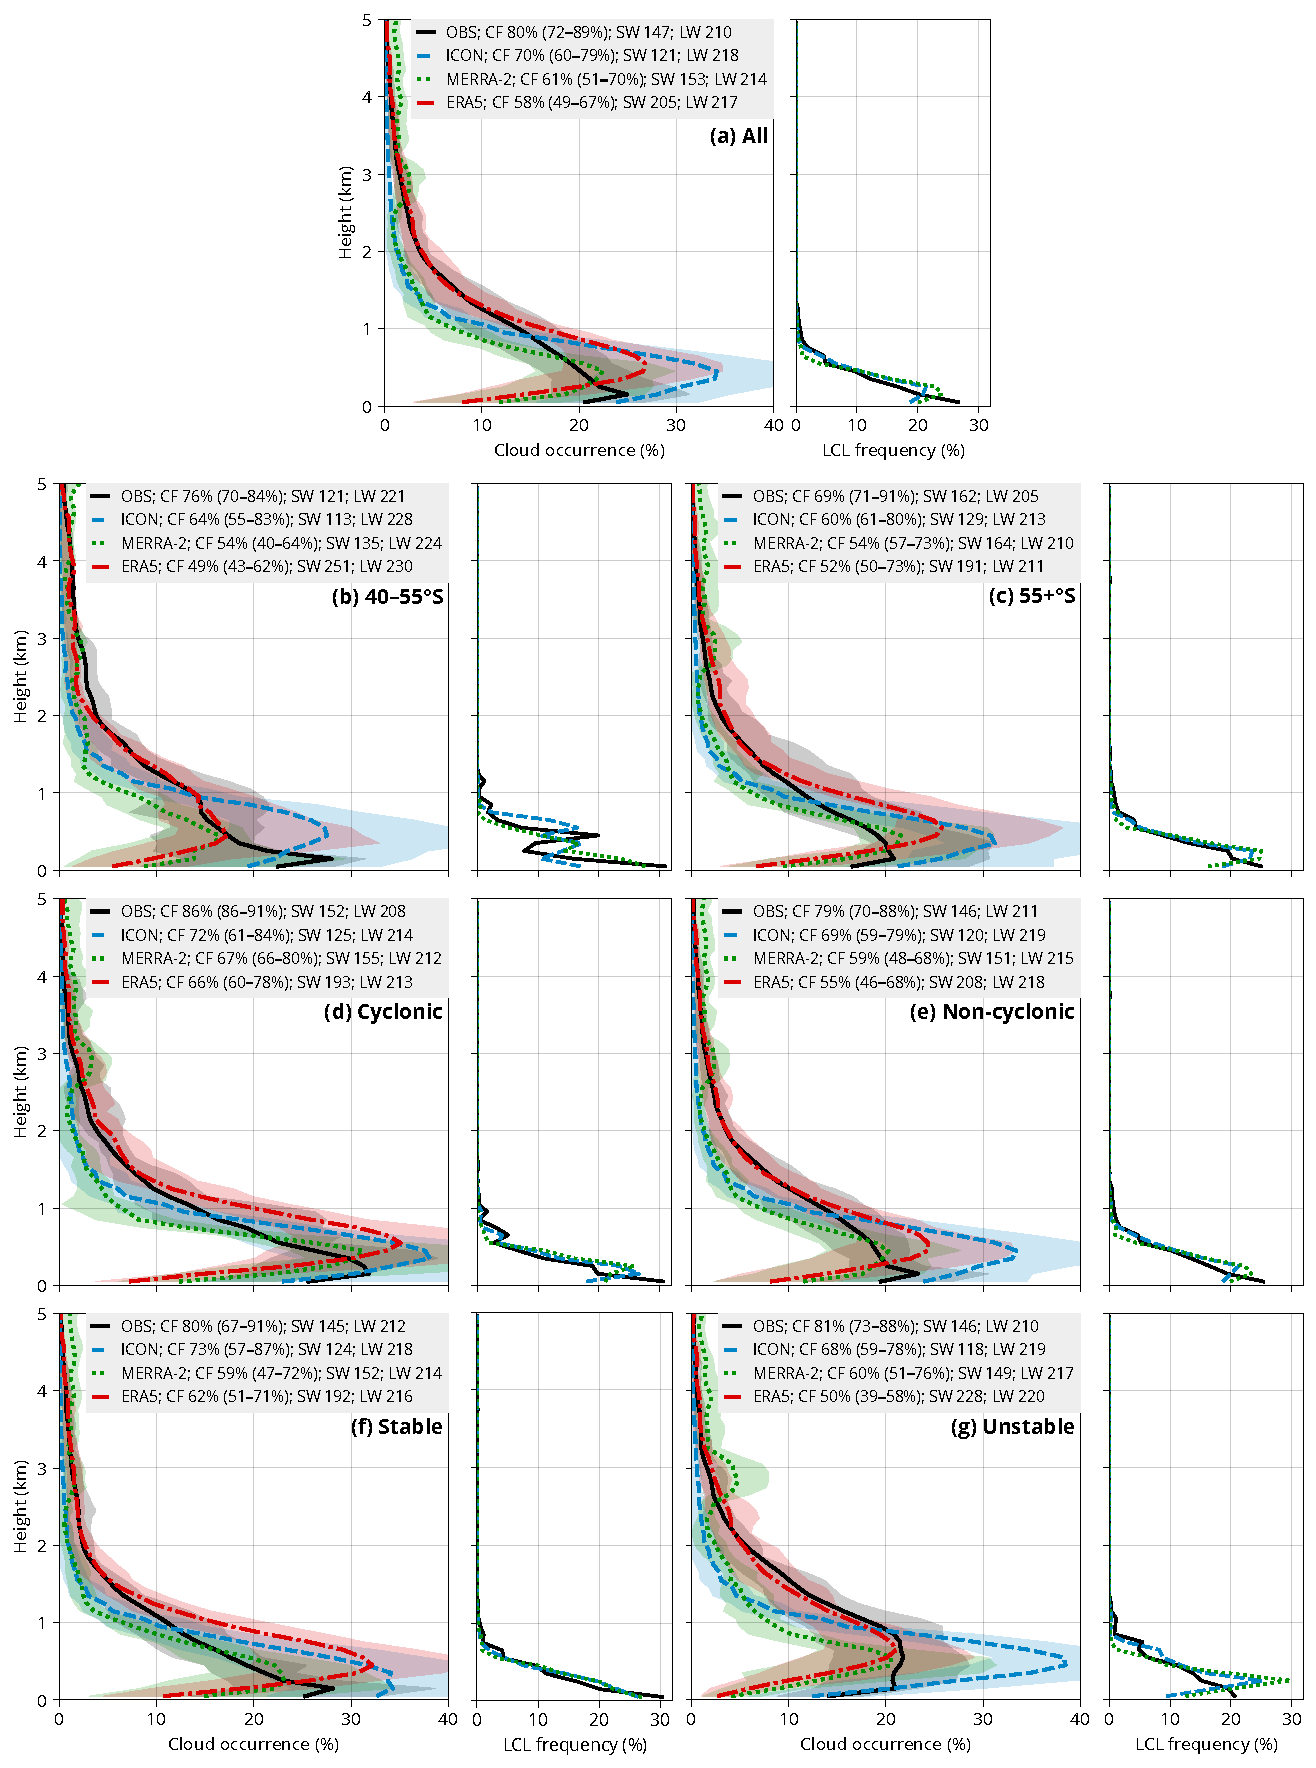
\includegraphics[width=\textwidth]{img/cl_agg.pdf}
\caption{
Cloud occurrence by height calculated as the average of all voyages and
stations for the observed (OBS) and simulated lidar cloud mask, and lifting
condensation level (LCL) distribution. The total cloud fraction (CF), average
shortwave (SW), and longwave (LW) are shown in the legend, and the relative
frequency of occurrence (RFO) of the subset is shown below.  The bands span the
16$^\mathrm{th}$--84$^\mathrm{th}$ percentile calculated from the set of all
voyages and stations. The subsets \textbf{(d--g)} are defined in Section
\ref{sec:cyclone-stability}.
}
\label{fig:cloud-occurrence}
\end{figure}

\subsection{Cloud cover}
\label{sec:cloud-cover}

We analysed the daily cloud cover (total cloud fraction) distribution. This is
a measure of cloudiness, irrespective of height, calculated over the course of
a day (UTC). A cloud detected at any height means that the lidar profile was
classified as cloudy; otherwise, it was classified as a clear sky. When all
profiles in a day are taken together, the cloud cover for the day is defined as
the fraction of cloudy profiles in the total number of profiles, expressed in
oktas (multiples of 1/8).

In Fig.  \ref{fig:cloud-cover} we show the results for the same subsets of data
as in the previous section. Observations have the greatest representation of
high cloud cover (5--8 oktas), peaking at 7 oktas. This is not represented by
ICON or the reanalyses.  While ICON is the closest, it tends to be 1 okta
clearer than the observations, peaking at 6 oktas, and highly underestimating
days with 8 oktas.  Overall, the reanalyses show results similar to each other,
underestimating cloud cover by about 2 oktas and strongly underestimating days
with 7 and 8 oktas. Of the two reanalyses, MERRA-2 shows slightly higher cloud
cover and thus is more consistent with observations.

When analysed by subsets, observations in the cyclonic subset show the highest
cloud cover, with 8 oktas occurring on one half of such days (Fig.
\ref{fig:cloud-cover}d).  This is not represented by ICON or the reanalyses at
all. Interestingly, clear sky days (0 oktas) also have a local maximum peaking
at about 15\% in this subset.  When we contrast the low- and high-latitude
zones, we see that the high-latitude zone tends to have greater cloud cover,
peaking at 8 oktas (Fig.  \ref{fig:cloud-cover}c). The high-latitude zone also
has almost no clear sky or small cloud cover cases (0--4 oktas). ICON and the
reanalyses represent at least this characteristic of the distribution well for
0--3 oktas, but otherwise show biases similar to the general case. One of the
greatest biases is present in ERA5 in the relatively unstable subset, in which
ERA5 peaks at 3 oktas, whereas the observations peak at 7 oktas and show
negligible cloud cover below 5 oktas.

\begin{figure}[p!]
\centering
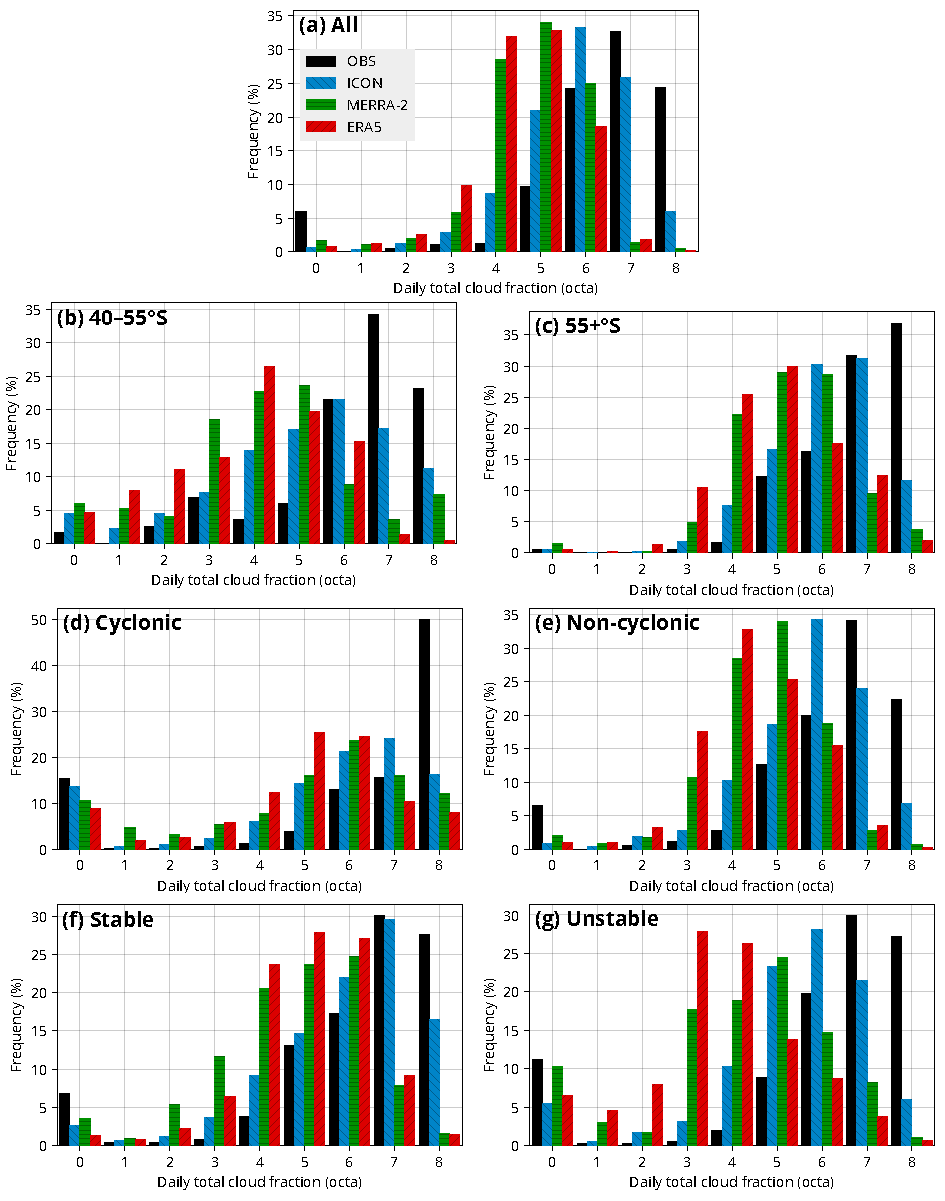
\includegraphics[width=\textwidth]{img/clt_hist.pdf}
\caption{
Daily total cloud fraction histograms calculated as the average of all voyage
and station histograms. The total cloud fraction of a day (UTC) is calculated
as a fraction of cloudy (based on the cloud mask) observed (OBS) or simulated
lidar profiles. The models and subsets are as in Fig.
\ref{fig:cloud-occurrence}.
}
\label{fig:cloud-cover}
\end{figure}

\begin{figure}[p!]
\centering
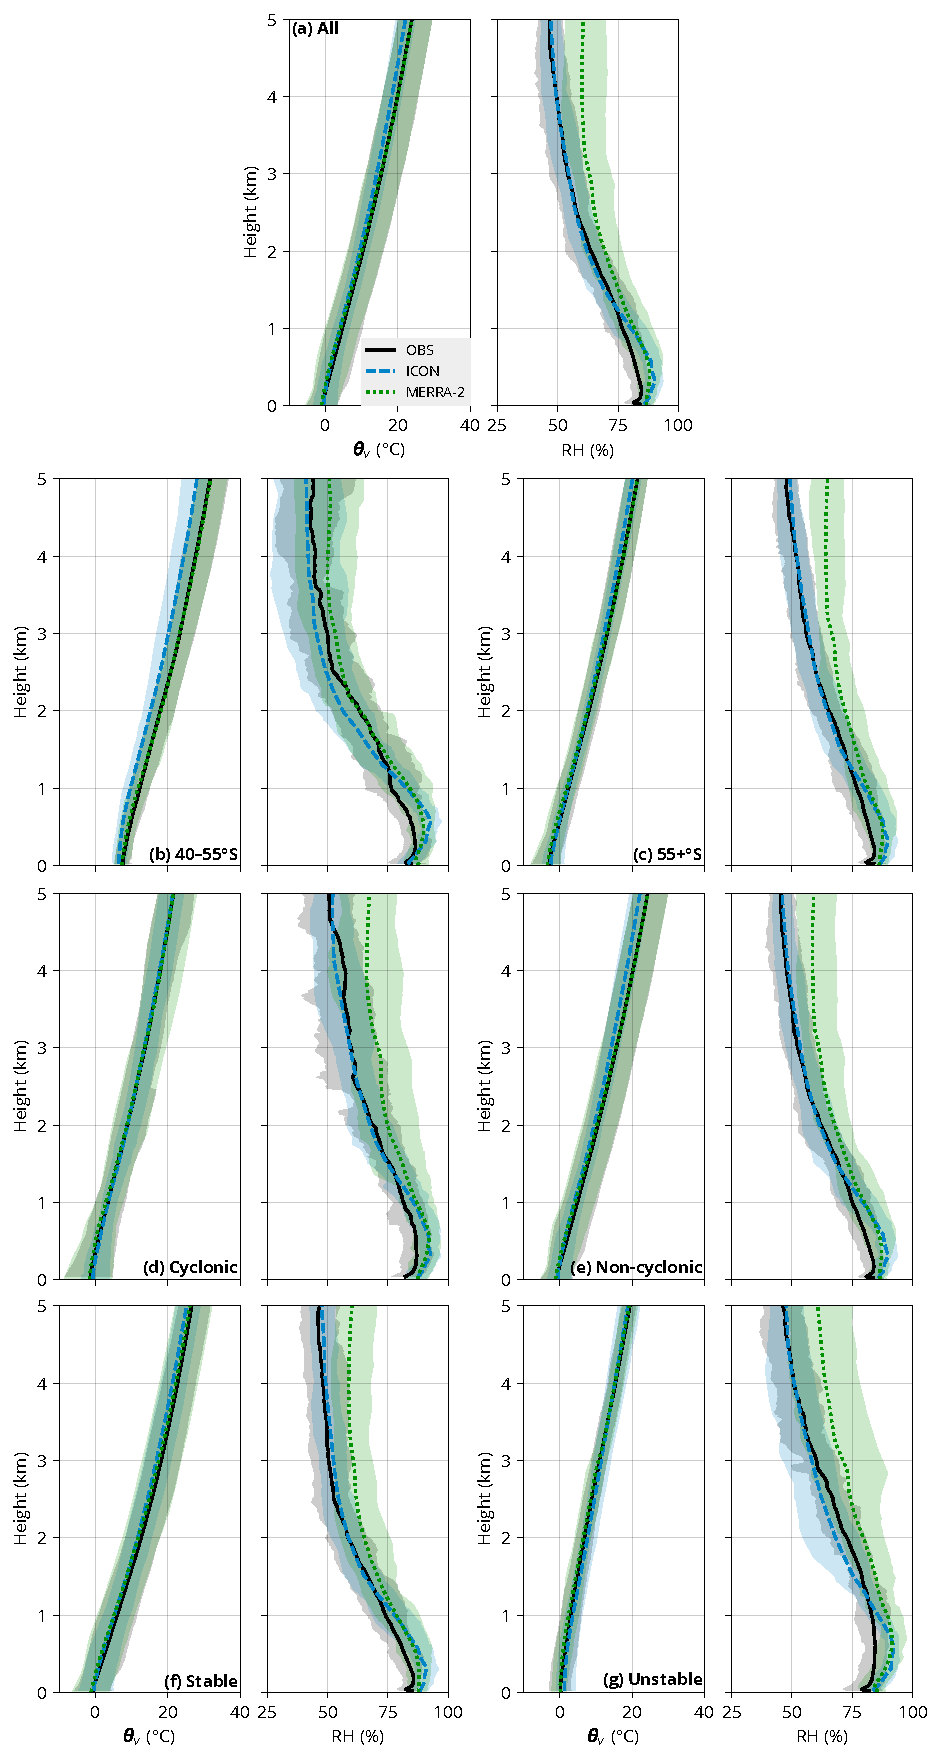
\includegraphics[width=0.72\textwidth]{img/theta_hur.pdf}
\caption{
Virtual potential temperature ($\theta_v$) and relative humidity (RH)
determined from radiosonde launches and co-located profiles in
ICON, ERA5, and MERRA-2 in subsets as in Fig. \ref{fig:cloud-occurrence}.
The solid lines are the average calculated from the averages of every
individual voyage and station. The bands span the
16$^\mathrm{th}$--84$^\mathrm{th}$ percentiles calculated from the distribution
of the voyage and station averages. Shown is also the relative frequency of
occurrence and the number of profiles in each subset.
}
\label{fig:potential-temperature}
\end{figure}

\subsection{Thermodynamic profiles}

We analysed about 2300 radiosonde profiles south of 40°S from the 24 RV
\emph{Polarstern} voyages, MARCUS, NBP1704, TAN1702, and TAN1802. Spatially and
temporally colocated profiles were taken from ICON and the reanalyses. Because
the time period of the ICON model output was different from the observations,
model time was chosen to be the same as the radiosonde launch time relative to
the start of the year. The profiles were partitioned into the same subsets as
above (Sections \ref{sec:cloud-occurrence} and \ref{sec:cloud-cover}).  Apart
from relative humidity, we focus on comparing virtual potential temperature
($\theta_v$) due to its role in low-level tropospheric stability, being one of
the primary factors affecting shallow convection and the associated low-level
cloud formation and dissipation. The observed and model profiles of virtual
potential temperature are shown in Fig. \ref{fig:potential-temperature}.

Overall, the mean $\theta_v$ is relatively well represented in ICON and
MERRA-2, being only slightly colder in the mid-to-high troposphere (less
stable) in ICON than in observations (Fig. \ref{fig:potential-temperature}a).
Large differences exist, however, in the 40--55°S zone, where ICON is colder in
$\theta_v$ by up to about 5 K and more so at higher altitudes (Fig.
\ref{fig:potential-temperature}b). In other subsets, the bias is relatively
small. MERRA-2 is very close to the observations, possibly due to a high
accuracy of assimilation of this quantity. Notably, the variability of virtual
potential temperature (as represented by the percentiles) is much smaller in
ICON than in the observations. This indicates that the model's internal
variability in the lower-tropospheric thermodynamic conditions in the SO is
smaller than in reality.

Relative humidity displays much larger biases. In all subsets, ICON is too
humid in the first 1 km but very accurate above, except for the 40--55°S zone
and unstable conditions (Fig. \ref{fig:potential-temperature}b, g),  where it
is too dry between about 1 and 3 km. MERRA-2, on the other hand, is much more
humid than observations at all altitudes and in all subsets, by up to about
20\% at 5 km.

\section{Limitations}

Let us consider the main limitations of the presented results. The spatial
coverage of our dataset does not include most parts of the Indian Ocean and
Pacific Ocean sectors of the SO. Even though climatological features of the SO
are typically relatively uniform zonally, variations exist, such as those
related to the Antarctic Peninsula and the southern tip of South America. The
voyages were mostly undertaken in the Austral summer months and only rarely in
the winter months, due to the poor accessibility of this region during winter.
Therefore, our results are mostly representative of summer and to a lesser
extent, spring and autumn conditions.

The time period of ICON is relatively short, with only four full years of
simulation available. Moreover, the simulation is free-running, which means
that observations had to be temporally mapped to this time period (at the same
time relative to the start of the year) for the comparison. For these reasons,
one can expect the results to be slightly different due to reasons unrelated to
model biases, such as different weather conditions and the phase of climate
oscillations such as the ENSO in the observations and the model.

Ground-based lidar observations are affected by attenuation by thick cloud
layers, and for this reason the results are mostly representative of boundary
layer clouds, while higher-level clouds are only occasionally visible to the
lidar when boundary layer clouds are not present. Ground-based lidar
observations can be regarded as superior to satellite lidar observations for
low-level clouds, which are predominant in this region, while mid- and
high-level clouds are better represented in satellite observations
\citep{mcerlich2021}.

We attempted to remove lidar profiles with precipitation, which could not be
properly simulated with the lidar simulator (Section \ref{sec:ann}). However,
the approach was limited by the relatively low sensitivity of the ANN (65\%)
and the fact that we had to choose a fixed threshold for surface precipitation
flux in the model and reanalyses, which might not exactly correspond to
detection by the ANN applied to observations. Also, we did not make an attempt
to remove profiles with precipitation not reaching the surface. The above
reasons can result in an artificial bias in the comparison, even though we
expect this to be much smaller than the identified model biases.

\section{Discussion and conclusions}

We analysed a total of about 2400 days of lidar and 2300 radiosonde
observations from 31 voyages/campaigns and a subantarctic station, covering the
Atlantic, Australian, and New Zealand sectors of the SO over the span of 10
years. This dataset, together with the use of a ground-based lidar simulator,
provided a comprehensive basis for evaluating SO cloud and thermodynamic
profile biases in the GSRM ICON and the ERA5 and MERRA-2 reanalyses. Our
analysis provides a unique evaluation perspective different from satellite
observations -- one that is more suitable for evaluating boundary layer clouds,
which are predominant in this region. Furthermore, we subsetted our dataset by
low and high latitude bands, cyclonic activity, and stability in order to
identify how these conditions relate to the biases.

Our main finding corroborates previous findings of large boundary layer cloud
biases in models and their subsequent effect on the radiative transfer. This
also applies to the new GSRM ICON, but the biases are lower than in the
reanalyses, despite the reanalyses having the advantage of assimilation of the
observed meteorological conditions.  The GSRM has, on the other hand, the
advantage of a much higher spatial resolution and, to a limited extent,
explicit calculation of traditionally subgrid-scale processes such as
convection.

We show that relative to ERA5, the distribution and strength of cyclonic
activity over the SO is well represented in ICON, but it is substantially less
stable in terms of LTS. The latter is also manifested in the radiosonde profile
comparison, showing that the virtual potential temperature profiles in ICON
are less stable than in the observations over low-latitude SO.

The 31 voyages and a station show fairly similar biases in cloud occurrence by
height in the lidar comparison, which indicates that common underlying causes
for the biases exist regardless of longitude and season. ICON underestimates
the total cloud fraction by about 10\%, with an overestimation of clouds below
2 km and an underestimation of clouds above 2 km. The reanalyses also
underestimate the total cloud fraction by about 20\%.  ERA5 overestimates cloud
below 1 km but underestimates near-surface cloud or fog. ICON strongly
overestimates the peak of cloud occurrence at about 500 m, which might be
explained by the radiosonde comparison, showing that it is too moist at
around this height.  Similar to our results, \cite{cesana2022} showed that
CMIP6 models also tend to underestimate cloud occurrence above 2 km over the
SO, although their analysis in this case was limited to liquid clouds.

Compared to lidar observations, the daily cloud cover tends to be about 1 okta
lower in ICON and 2 oktas lower in the reanalyses.  Unstable conditions are
associated with some of the greatest biases, especially in ERA5.  The models
also underestimate the cloud cover very strongly in cyclonic conditions, which
are very cloudy in the observations (8 oktas), but much less so in the models.

The radiosonde observations indicate that the LCL is too high in ICON and
reanalyses, which is probably responsible for the higher peak of clouds in the
models and the lack of near-surface clouds or fog. The radiosonde comparison,
however, does not seem to explain cloud biases at higher altitudes.  MERRA-2 is
too moist at all heights.  ICON also exhibits smaller internal variability than
the radiosonde observations. Overall, the radiosonde comparison is only
partially explaining the identified cloud biases, and other physical causes are
likely contributing.  This warrants further investigation, especially of
ocean--atmosphere fluxes, shallow convection, and boundary layer turbulence.
The lack of parametrised subgrid-scale convection in ICON might be a
substantial issue even at the 5-km resolution.

The relationship between cloud biases and radiation has a number of notable
features. Perhaps unsurprisingly, the reanalyses exhibit the too few, too
bright bias previously identified in models. In our results, this is
characterised by outgoing TOA SW radiation similar to or higher than in the
satellite observations, while at the same time total cloud fraction is
substantially underestimated relative to the ground-based lidar observations.
This feature seems to be much more pronounced in ERA5 than in MERRA-2. On the
other hand, this type of relationship is not present in ICON. This model mostly
predicts smaller outgoing TOA SW radiation and smaller total cloud fraction
than observations, and the deficit of outgoing TOA SW radiation is
approximately proportional to the deficit of the total cloud fraction. While this
might be a welcome feature and an improvement over previous models, it does
mean that the outgoing TOA SW radiation is overall underestimated instead of
being compensated by a higher cloud albedo. This can, of course, lead to
undesirable secondary effects such as overestimated solar heating of the sea
surface, among other factors responsible for SO SST biases in climate models
\citep{zhang2023,luo2023}.

The results imply that SO cloud biases are still a substantial issue in the
km-scale resolution ICON model, even though an improvement over the
lower-resolution reanalyses is notable. More effort is needed to improve the
model cloud simulations in this fast-changing and understudied region. The
transition from models with parametrised convection and clouds to
storm-resolving models might not solve these biases without additional effort.
Evaluation of ocean--atmosphere heat, moisture, and momentum fluxes against in
situ observations over the SO and comparison of GSRM simulations against
large-eddy simulations are two potential avenues for future research that could
elucidate the physical mechanisms behind the biases, in addition to the more
common efforts in SO cloud microphysics and precipitation evaluation.

\fontsize{12pt}{14pt}\selectfont
\section*{Acknowledgements}

PK and FB, and the nextGEMS project received funding from the European Union’s
Horizon 2020 research and innovation program under a grant agreement no.
101003470. FB received funding from the Wenner-Gren Foundation and the Swedish
e-Science Research Centre.  The work of GM was supported by the United States
(U.S.) Department of Energy Award DE-SC0021159.  Supercomputing resources were
provided by the DKRZ (project 1125 ICON-development) and the National Academic
Infrastructure for Supercomputing in Sweden (allocation 2023/22-202). The data
collection by the University of Canterbury was funded by the Deep South
National Science Challenge Clouds and Aerosols project.  Data collection on the
AA15-16 voyages was funded by the Australian Antarctic Science project (grant
no.  4292).  We acknowledge the contribution of Thorsten Mauritsen to funding
acquisition and project management.  We acknowledge the RV \emph{Polarstern}
datasets provided by the Alfred Wegener Institute and Pangaea, the AA15-16
dataset provided by the Australian Antarctic Division (AAD) and University of
Canterbury (UC), the RV \emph{Tangaroa} datasets provided by the National Institute
of Water and Atmospheric Research and UC, the NBP1704 dataset provided by the
National Science Foundation, Cooperative Institute for Research in
Environmental Sciences, University of Colorado and UC, the HMNZSW16 dataset
provided by the Royal New Zealand Navy and UC, the MARCUS dataset provided by
the Atmospheric Radiation Measurement (ARM) and AAD, and the MICRE dataset
provided by ARM, the Australian Bureau of Meteorology, and AAD.  Technical,
logistical, and ship support for MARCUS and MICRE were provided by the AAD
through Australian Antarctic Science projects 4292 and 4387, and we thank
Steven Whiteside, Lloyd Symonds, Rick van den Enden, Peter de Vries, Chris
Young, Chris Richards, Andrew Klekociuk, John French, Terry Egan, Nick
Cartwright, and Ken Barrett for all of their assistance.  We thank the
scientific staff, the crew, and everyone involved in collecting data on the
voyages and stations, especially Gert König-Langlo, Holger Schmithüsen, Roger
Marchand, Peter Guest, Kelly Schick, Jamie Halla, and Mike J.  Harvey (†). We
thank Loretta Preis for providing additional RV \emph{Polarstern} data.  We
acknowledge the ICON model output provided by the nextGEMS project, Deutscher
Wetterdienst, Max-Planck-Institute for Meteorology, DKRZ, Karlsruhe Institute
of Technology, and Center for Climate Systems Modeling; reanalysis dataset ERA5
provided by the Copernicus Climate Change Service; MERRA-2 provided by the
Global Modeling and Assimilation Office; CERES datasets provided by the NASA
Langley Atmospheric Science Data Center Distributed Active Archive Center; and
the Natural Earth dataset provided by naturalearthdata.com.  Last but not
least, we acknowledge the use of open source software Python, Cython
\citep{behnel2011}, TensorFlow \citep{abadi2016}, Devuan GNU+Linux, parallel
\citep{tange2011}, NumPy \citep{harris2020}, SciPy \citep{virtanen2020},
Matplotlib \citep{hunter2007}, cartopy \citep{cartopy}, pyproj, Inkscape, Bash,
GNU Fortran, HDF \citep{folk1999}, and NetCDF \citep{rew1990}.  We dedicate
this study to the memory of Mike J.  Harvey, who very substantially contributed
to obtaining the atmospheric observations on the RV \emph{Tangaroa} voyages
used in this study.

\section*{Code availability}

The ALCF, cl2nc, rstool, lidar precipitation detection code, and our data
processing and plotting code are open source and available at
\url{https://alcf.peterkuma.net}, \url{https://github.com/peterkuma/cl2nc},
\url{https://github.com/peterkuma/rstool}, and
\url{https://github.com/peterkuma/alcf-precip},
\url{https://github.com/peterkuma/icon-so-2024}, respectively. CyTRACK is
available at \url{https://github.com/apalarcon/CyTRACK}. The ICON model is
available at \url{https://gitlab.dkrz.de/icon/icon-mpim}.

\section*{Data availability}

The RV \emph{Polarstern} datasets are openly available on Pangaea
(\url{https://pangaea.de}). The MARCUS and MICRE datasets are openly available
from ARM (\url{https://www.arm.gov}). The MERRA-2 data are openly available
from the NASA Goddard Earth Sciences (GES) Data and Information Services Center
(DISC) (\url{https://disc.gsfc.nasa.gov/datasets?project=MERRA-2}).  The ERA5
data are openly available from the Copernicus Climate Data Store (CDS)
(\url{https://cds.climate.copernicus.eu}). The ICON data are available on the
Levante cluster of the DKRZ
(\url{https://www.dkrz.de/en/systems/hpc/hlre-4-levante}) after registration at
\url{https://luv.dkrz.de/register/}. The CERES products are available from the
project website (\url{https://ceres.larc.nasa.gov}) and the NASA Atmospheric
Science Data Centre (\url{https://asdc.larc.nasa.gov/project/CERES}).  The
TAN1802 data are available on Zenodo
(\url{https://doi.org/10.5281/zenodo.4060237}).

% TODO: The other voyage and station data are openly available on Zenodo ().
% Subsetted model and reanalysis data for the voyage tracks and the station and
% data processed with the ALCF are openly available on Zenodo ().

\section*{Author contributions}

The authors have made the following contributions based on the CRediT taxonomy
(\url{https://credit.niso.org}).  PK: conceptualization, data curation, formal
analysis, investigation, methodology, software, writing – original draft; FAMB:
conceptualization, funding acquisition, project administration, supervision,
and writing – review \& editing; AJM, SPA, GMM, JJC, GEP, SH, SP, SG, and AJS:
data curation, investigation, resources, writing – review \& editing.

%\footnotesize
\fontsize{11pt}{13pt}\selectfont
\setlength{\bibsep}{0.0pt}
\bibliography{manuscript}

\end{document}
